% =============================================================================
%  Tài liệu sản phẩm --- da2: Triển khai mô hình SVM chẩn đoán ung thư vú
%
%  Biên dịch:  latexmk -pdf da2_tai_lieu_san_pham.tex        (pdfLaTeX)
%  Trên Overleaf:  Menu > Compiler > pdfLaTeX  (dùng gói docs/latex/da2_tai_lieu_overleaf.zip)
%
%  KHÔNG dùng XeLaTeX cho tệp này: gói `vietnam` (vntex) là gói 8-bit, chỉ chạy
%  với pdfLaTeX. Riêng da2_slide.tex dùng XeLaTeX (fontspec).
%
%  Số liệu trong tài liệu lấy tự động từ metrics_data.tex, sinh bằng:
%      python docs/latex/make_tex_data.py
% =============================================================================
\documentclass[12pt]{article}
\usepackage[a4paper]{geometry}
\usepackage[utf8]{vietnam}

\usepackage{graphicx}
\usepackage{caption}
\usepackage{float}

\usepackage{indentfirst}
\usepackage{amsmath}
\usepackage{amssymb}
\usepackage{anysize}
\marginsize{2cm}{2cm}{2cm}{1.5cm} % {trái}{phải}{trên}{dưới}
\usepackage{parskip}
\usepackage[colorlinks = false, plainpages = false]{hyperref}
\usepackage{xurl}

\usepackage{xcolor}
\definecolor{codegreen}{rgb}{0,0.6,0}
\definecolor{codegray}{rgb}{0.5,0.5,0.5}
\definecolor{codepurple}{rgb}{0.58,0,0.82}
\definecolor{backcolour}{rgb}{0.95,0.95,0.92}
\definecolor{warnbg}{RGB}{255,244,229}

\usepackage{listings}
\lstdefinestyle{mystyle}{
    backgroundcolor=\color{backcolour},
    commentstyle=\color{codegreen},
    keywordstyle=\color{blue},
    numberstyle=\tiny\color{codegray},
    stringstyle=\color{codepurple},
    basicstyle=\ttfamily\footnotesize,
    breakatwhitespace=false,
    breaklines=true,
    captionpos=b,
    keepspaces=true,
    numbers=left,
    numbersep=5pt,
    showspaces=false,
    showstringspaces=false,
    showtabs=false,
    tabsize=4,
    frame=single,
    rulecolor=\color{codegray},
    language=Python,
}
\lstset{style=mystyle}

% Xử lý tiếng Việt trong code: bảng ánh xạ sinh bằng docs/latex/make_listings_map.py
% (gói Overleaf nhúng sẵn bảng tối thiểu, xem build_overleaf.py)
% =============================================================================
%  Tệp sinh tự động bởi docs/make_listings_map.py — KHÔNG sửa tay.
%
%  pdfLaTeX không đọc được UTF-8 bên trong lstlisting, nên mọi ký tự có dấu trong
%  mã nguồn Python phải được ánh xạ sang lệnh đặt dấu của bảng mã T5 (gói vietnam).
% =============================================================================
\lstset{literate=%
    {±}{{$\pm$}}1 {²}{{$^2$}}1 {·}{{$\cdot$}}1 {À}{{\`{A}}}1 %
    {Á}{{\'{A}}}1 {Â}{{\^{A}}}1 {Ã}{{\~{A}}}1 {È}{{\`{E}}}1 %
    {É}{{\'{E}}}1 {Ê}{{\^{E}}}1 {Ì}{{\`{I}}}1 {Í}{{\'{I}}}1 %
    {Î}{{\^{I}}}1 {Ò}{{\`{O}}}1 {Ó}{{\'{O}}}1 {Ô}{{\^{O}}}1 %
    {Õ}{{\~{O}}}1 {×}{{$\times$}}1 {Ù}{{\`{U}}}1 {Ú}{{\'{U}}}1 %
    {Û}{{\^{U}}}1 {Ý}{{\'{Y}}}1 {à}{{\`{a}}}1 {á}{{\'{a}}}1 %
    {â}{{\^{a}}}1 {ã}{{\~{a}}}1 {è}{{\`{e}}}1 {é}{{\'{e}}}1 %
    {ê}{{\^{e}}}1 {ì}{{\`{i}}}1 {í}{{\'{i}}}1 {î}{{\^{i}}}1 %
    {ò}{{\`{o}}}1 {ó}{{\'{o}}}1 {ô}{{\^{o}}}1 {õ}{{\~{o}}}1 %
    {ù}{{\`{u}}}1 {ú}{{\'{u}}}1 {û}{{\^{u}}}1 {ý}{{\'{y}}}1 %
    {Ă}{{\u{A}}}1 {ă}{{\u{a}}}1 {Đ}{{\DJ}}1 {đ}{{\dj}}1 %
    {Ĕ}{{\u{E}}}1 {ĕ}{{\u{e}}}1 {Ĩ}{{\~{I}}}1 {ĩ}{{\~{i}}}1 %
    {Ĭ}{{\u{I}}}1 {ĭ}{{\u{i}}}1 {Ŏ}{{\u{O}}}1 {ŏ}{{\u{o}}}1 %
    {Ũ}{{\~{U}}}1 {ũ}{{\~{u}}}1 {Ŭ}{{\u{U}}}1 {ŭ}{{\u{u}}}1 %
    {Ŷ}{{\^{Y}}}1 {ŷ}{{\^{y}}}1 {Ơ}{{\OHORN}}1 {ơ}{{\ohorn}}1 %
    {Ư}{{\UHORN}}1 {ư}{{\uhorn}}1 {γ}{{$\gamma$}}1 {Ṍ}{{\'{O}}}1 %
    {ṍ}{{\'{o}}}1 {Ṹ}{{\'{U}}}1 {ṹ}{{\'{u}}}1 {Ạ}{{\d{A}}}1 %
    {ạ}{{\d{a}}}1 {Ả}{{\h{A}}}1 {ả}{{\h{a}}}1 {Ấ}{{\'{\^{A}}}}1 %
    {ấ}{{\'{\^{a}}}}1 {Ầ}{{\`{\^{A}}}}1 {ầ}{{\`{\^{a}}}}1 {Ẩ}{{\h{\^{A}}}}1 %
    {ẩ}{{\h{\^{a}}}}1 {Ẫ}{{\~{\^{A}}}}1 {ẫ}{{\~{\^{a}}}}1 {Ậ}{{\d{\^{A}}}}1 %
    {ậ}{{\d{\^{a}}}}1 {Ắ}{{\'{\u{A}}}}1 {ắ}{{\'{\u{a}}}}1 {Ằ}{{\`{\u{A}}}}1 %
    {ằ}{{\`{\u{a}}}}1 {Ẳ}{{\h{\u{A}}}}1 {ẳ}{{\h{\u{a}}}}1 {Ẵ}{{\~{\u{A}}}}1 %
    {ẵ}{{\~{\u{a}}}}1 {Ặ}{{\d{\u{A}}}}1 {ặ}{{\d{\u{a}}}}1 {Ẹ}{{\d{E}}}1 %
    {ẹ}{{\d{e}}}1 {Ẻ}{{\h{E}}}1 {ẻ}{{\h{e}}}1 {Ẽ}{{\~{E}}}1 %
    {ẽ}{{\~{e}}}1 {Ế}{{\'{\^{E}}}}1 {ế}{{\'{\^{e}}}}1 {Ề}{{\`{\^{E}}}}1 %
    {ề}{{\`{\^{e}}}}1 {Ể}{{\h{\^{E}}}}1 {ể}{{\h{\^{e}}}}1 {Ễ}{{\~{\^{E}}}}1 %
    {ễ}{{\~{\^{e}}}}1 {Ệ}{{\d{\^{E}}}}1 {ệ}{{\d{\^{e}}}}1 {Ỉ}{{\h{I}}}1 %
    {ỉ}{{\h{i}}}1 {Ị}{{\d{I}}}1 {ị}{{\d{i}}}1 {Ọ}{{\d{O}}}1 %
    {ọ}{{\d{o}}}1 {Ỏ}{{\h{O}}}1 {ỏ}{{\h{o}}}1 {Ố}{{\'{\^{O}}}}1 %
    {ố}{{\'{\^{o}}}}1 {Ồ}{{\`{\^{O}}}}1 {ồ}{{\`{\^{o}}}}1 {Ổ}{{\h{\^{O}}}}1 %
    {ổ}{{\h{\^{o}}}}1 {Ỗ}{{\~{\^{O}}}}1 {ỗ}{{\~{\^{o}}}}1 {Ộ}{{\d{\^{O}}}}1 %
    {ộ}{{\d{\^{o}}}}1 {Ớ}{{\'{\OHORN}}}1 {ớ}{{\'{\ohorn}}}1 {Ờ}{{\`{\OHORN}}}1 %
    {ờ}{{\`{\ohorn}}}1 {Ở}{{\h{\OHORN}}}1 {ở}{{\h{\ohorn}}}1 {Ỡ}{{\~{\OHORN}}}1 %
    {ỡ}{{\~{\ohorn}}}1 {Ợ}{{\d{\OHORN}}}1 {ợ}{{\d{\ohorn}}}1 {Ụ}{{\d{U}}}1 %
    {ụ}{{\d{u}}}1 {Ủ}{{\h{U}}}1 {ủ}{{\h{u}}}1 {Ứ}{{\'{\UHORN}}}1 %
    {ứ}{{\'{\uhorn}}}1 {Ừ}{{\`{\UHORN}}}1 {ừ}{{\`{\uhorn}}}1 {Ử}{{\h{\UHORN}}}1 %
    {ử}{{\h{\uhorn}}}1 {Ữ}{{\~{\UHORN}}}1 {ữ}{{\~{\uhorn}}}1 {Ự}{{\d{\UHORN}}}1 %
    {ự}{{\d{\uhorn}}}1 {Ỳ}{{\`{Y}}}1 {ỳ}{{\`{y}}}1 {Ỵ}{{\d{Y}}}1 %
    {ỵ}{{\d{y}}}1 {Ỷ}{{\h{Y}}}1 {ỷ}{{\h{y}}}1 {Ỹ}{{\~{Y}}}1 %
    {ỹ}{{\~{y}}}1 {–}{{--}}2 {—}{{---}}3 {“}{{``}}1 %
    {”}{{''}}1 {…}{{\dots}}3 {→}{{$\rightarrow$}}2 {−}{{$-$}}1 %
    {∞}{{$\infty$}}1 {≠}{{$\neq$}}1 {≤}{{$\leq$}}1 {≥}{{$\geq$}}1 %
    {✔}{{$\checkmark$}}1
}


\setlength{\parskip}{8pt}

\usepackage{tikz}
\usetikzlibrary{calc,positioning,arrows.meta}

% Nơi tìm hình: kho mã nguồn khi build ở máy; trong gói Overleaf mọi hình nằm cạnh main.tex
\graphicspath{{../../reports/figures/}{../screenshots/}{./}}

% Địa chỉ dịch vụ trên Render xuất hiện nguyên văn (macro không mở rộng trong \url và lstlisting):
% đổi bằng  python docs/latex/set_service_url.py <URL mới>

\newtheorem{definition}{Định nghĩa}[subsection]
\newcommand{\R}{\mathbb{R}}

\usepackage{sectsty}
\subsubsectionfont{\normalfont\itshape}

\usepackage{booktabs}
\captionsetup{skip=0.333\baselineskip}

\newcommand{\canhbao}[1]{\par\noindent\colorbox{warnbg}{\parbox{\dimexpr\linewidth-2\fboxsep}{#1}}\par}

% Tệp sinh tự động bởi docs/latex/make_tex_data.py — KHÔNG sửa tay.
% Nguồn: reports/metrics.json + artifacts/metadata.json (train lúc 2026-09-26T12:35:51+00:00)

\newcommand{\GeneratedAt}{2026-09-26 12:35:51 U C}
\newcommand{\ModelName}{\texttt{breast-cancer-svm-rbf}}
\newcommand{\ModelVersion}{1.0.0}
\newcommand{\SklearnVersion}{1.9.1}
\newcommand{\NumpyVersion}{2.5.3}
\newcommand{\PythonVersion}{3.12.10}
\newcommand{\DataHashShort}{25e2eb7b7a87}
\newcommand{\NSamples}{569}
\newcommand{\NFeatures}{30}
\newcommand{\NMalignant}{212}
\newcommand{\NBenign}{357}
\newcommand{\PctMalignant}{37.3\%}
\newcommand{\PctBenign}{62.7\%}
\newcommand{\NTrain}{455}
\newcommand{\NTest}{114}
\newcommand{\TestMalignant}{42}
\newcommand{\TestBenign}{72}
\newcommand{\NZeroRows}{13}
\newcommand{\NZeroFeatures}{6}
\newcommand{\ZeroFeatures}{\texttt{mean concavity}, \texttt{mean concave points}, \texttt{concavity error}, \texttt{concave points error}, \texttt{worst concavity}, \texttt{worst concave points}}
\newcommand{\RandomState}{42}
\newcommand{\UpperFactor}{3}
\newcommand{\PcaOne}{44.3\%}
\newcommand{\PcaTwo}{19.0\%}
\newcommand{\PcaTotal}{63.2\%}
\newcommand{\GridConfigs}{16}
\newcommand{\GridSeconds}{2.8}
\newcommand{\GridScoring}{\texttt{recall\_macro}}
\newcommand{\BestC}{10}
\newcommand{\BestGamma}{0.01}
\newcommand{\GridCVMean}{0.9753}
\newcommand{\GridCVStd}{0.0162}
\newcommand{\CalibChosen}{\texttt{calibrated\_sigmoid\_single}}
\newcommand{\CalibChosenBrier}{0.01903}
\newcommand{\CalibBaselineBrier}{0.01873}
\newcommand{\CalibSigmoidBrier}{0.02476}
\newcommand{\CalibIsotonicBrier}{0.01956}
\newcommand{\Threshold}{0.3993}
\newcommand{\TargetSens}{0.97}
\newcommand{\ImpliedCostRatio}{1.50}
\newcommand{\TrainSens}{0.9824}
\newcommand{\TrainSpec}{0.9895}
\newcommand{\CVSens}{0.9706}
\newcommand{\CVSpec}{0.9789}
\newcommand{\CVTP}{165}
\newcommand{\CVFN}{5}
\newcommand{\CVFP}{6}
\newcommand{\CVHalfSens}{0.9647}
\newcommand{\CVHalfSpec}{0.9860}
\newcommand{\CVHalfTP}{164}
\newcommand{\CVHalfFN}{6}
\newcommand{\CVHalfFP}{4}
\newcommand{\CVMalignant}{170}
\newcommand{\TestSens}{0.9762}
\newcommand{\TestSpec}{0.9306}
\newcommand{\TestPrec}{0.8913}
\newcommand{\TestFOne}{0.9318}
\newcommand{\TestNPV}{0.9853}
\newcommand{\TestAcc}{0.9474}
\newcommand{\TestAUC}{0.9967}
\newcommand{\TestPRAUC}{0.9952}
\newcommand{\TestBrier}{0.0235}
\newcommand{\TestTP}{41}
\newcommand{\TestFN}{1}
\newcommand{\TestFP}{5}
\newcommand{\TestTN}{67}
\newcommand{\HalfSens}{0.9762}
\newcommand{\HalfSpec}{0.9722}
\newcommand{\HalfPrec}{0.9535}
\newcommand{\HalfFN}{1}
\newcommand{\HalfFP}{2}
\newcommand{\TestNErrors}{6}
\newcommand{\MissedProba}{0.0987}
\newcommand{\FPMinProba}{0.4617}
\newcommand{\FPMaxProba}{0.7249}
\newcommand{\FPBelowHalf}{3}

% Bảng so sánh cách hiệu chỉnh xác suất (4 cột)
\newcommand{\CalibRows}{%
  \texttt{svc\_probability} & 0.01873 & 0.07208 & 0.9958 & Platt trong libsvm, deprecated từ 1.9 \\
  \textbf{\texttt{calibrated\_sigmoid\_single}} & 0.01903 & 0.07381 & 0.9955 & khuyến nghị thay \texttt{probability=True} \\
  \texttt{calibrated\_sigmoid} & 0.02476 & 0.10639 & 0.9959 & trung bình 5 mô hình đã hiệu chỉnh \\
  \texttt{calibrated\_isotonic} & 0.01956 & 0.13740 & 0.9937 & hồi quy đơn điệu, không tham số \\
}

% Bảng metric train / CV / test (10 cột)
\newcommand{\MetricRows}{%
  Train & 0.3993 & 0.9824 & 0.9895 & 0.9824 & 0.9824 & 0.9983 & 0.9978 & 3 & 3 \\
  CV out-of-fold & 0.3993 & 0.9706 & 0.9789 & 0.9649 & 0.9677 & 0.9955 & 0.9946 & 5 & 6 \\
  \textbf{Test} & 0.3993 & 0.9762 & 0.9306 & 0.8913 & 0.9318 & 0.9967 & 0.9952 & 1 & 5 \\
  Test, ngưỡng 0.5 & 0.5000 & 0.9762 & 0.9722 & 0.9535 & 0.9647 & 0.9967 & 0.9952 & 1 & 2 \\
}

% Bảng metric rút gọn cho slide (6 cột)
\newcommand{\MetricRowsShort}{%
  Train & 0.9824 & 0.9895 & 0.9824 & 0.9983 & 3 \\
  CV (OOF) & 0.9706 & 0.9789 & 0.9649 & 0.9955 & 5 \\
  \textbf{Test} & 0.9762 & 0.9306 & 0.8913 & 0.9967 & 1 \\
  Test @ 0.5 & 0.9762 & 0.9722 & 0.9535 & 0.9967 & 1 \\
}

% Các mẫu test bị dự đoán sai (4 cột)
\newcommand{\ErrorRows}{%
  3 & lành tính & ác tính & 0.4617 \\
  16 & lành tính & ác tính & 0.7249 \\
  38 & lành tính & ác tính & 0.4707 \\
  51 & lành tính & ác tính & 0.4932 \\
  53 & ác tính & lành tính & 0.0987 \\
  66 & lành tính & ác tính & 0.5096 \\
}

% Kết quả GridSearchCV (4 cột)
\newcommand{\GridRows}{%
  10 & 0.01 & 0.9753 $\pm$ 0.0162 & 1 \\
  10 & 0.001 & 0.9736 $\pm$ 0.0059 & 2 \\
  1 & scale & 0.9730 $\pm$ 0.0107 & 3 \\
  1 & 0.01 & 0.9724 $\pm$ 0.0080 & 4 \\
  100 & 0.001 & 0.9724 $\pm$ 0.0080 & 4 \\
  100 & scale & 0.9666 $\pm$ 0.0232 & 6 \\
  10 & scale & 0.9654 $\pm$ 0.0089 & 7 \\
  1 & 0.1 & 0.9578 $\pm$ 0.0132 & 8 \\
  100 & 0.01 & 0.9577 $\pm$ 0.0133 & 9 \\
  10 & 0.1 & 0.9461 $\pm$ 0.0249 & 10 \\
  100 & 0.1 & 0.9461 $\pm$ 0.0249 & 10 \\
  0.1 & scale & 0.9449 $\pm$ 0.0121 & 12 \\
  1 & 0.001 & 0.9371 $\pm$ 0.0207 & 13 \\
  0.1 & 0.01 & 0.9330 $\pm$ 0.0206 & 14 \\
  0.1 & 0.1 & 0.9081 $\pm$ 0.0313 & 15 \\
  0.1 & 0.001 & 0.8624 $\pm$ 0.0428 & 16 \\
}

% ----- So sánh 5 mô hình phân loại (reports/comparison.json, train lúc 2026-09-27T06:34:11+00:00) -----
\newcommand{\CmpNModels}{5}
\newcommand{\CmpSeconds}{17.1}
\newcommand{\CmpBestLabel}{Logistic Regression}
\newcommand{\CmpBestCV}{0.9760}
\newcommand{\CmpBestCVStd}{0.0116}
\newcommand{\CmpSvmCV}{0.9753}
\newcommand{\CmpSvmCVStd}{0.0162}
\newcommand{\CmpGap}{0.0007}
\newcommand{\CmpBestSpec}{0.9861}
\newcommand{\CmpFastestLabel}{Logistic Regression}
\newcommand{\CmpFastestUs}{4.3}
\newcommand{\CmpSpeedFast}{1.5}
\newcommand{\CmpSpeedMedium}{3}

% Bảng so sánh (9 cột), dòng in đậm là mô hình có CV cao nhất
\newcommand{\CmpRows}{%
  \textbf{Logistic Regression} & 0.9760 & 0.9762 & 0.9861 & 0.9954 & 0.5783 & 1/1 & 9.7 & 4.3 \\
  SVM (RBF) & 0.9753 & 0.9762 & 0.9306 & 0.9967 & 0.3993 & 1/5 & 45.9 & 21.7 \\
  SVM tuyến tính & 0.9724 & 0.9762 & 0.9444 & 0.9960 & 0.3920 & 1/4 & 47.8 & 19.0 \\
  Random Forest & 0.9613 & 0.9524 & 0.9444 & 0.9945 & 0.4900 & 2/4 & 153.5 & 82.4 \\
  K láng giềng gần (KNN) & 0.9577 & 0.9762 & 0.8889 & 0.9944 & 0.3333 & 1/8 & 1.9 & 53.5 \\
}

% Bảng rút gọn cho slide (5 cột)
\newcommand{\CmpRowsShort}{%
  \textbf{Logistic Regression} & 0.9760 & 0.9762 & 0.9861 & 0.9954 \\
  SVM (RBF) & 0.9753 & 0.9762 & 0.9306 & 0.9967 \\
  SVM tuyến tính & 0.9724 & 0.9762 & 0.9444 & 0.9960 \\
  Random Forest & 0.9613 & 0.9524 & 0.9444 & 0.9945 \\
  K láng giềng gần (KNN) & 0.9577 & 0.9762 & 0.8889 & 0.9944 \\
}



\begin{document}

% ----------------------------------------------------------------------
% Trang bìa
% ----------------------------------------------------------------------
\thispagestyle{empty}
\begin{titlepage}

        \begin{tikzpicture}[overlay,remember picture]
        \draw [line width=3pt]
            ($ (current page.north west) + (1cm,-1cm) $)
            rectangle
            ($ (current page.south east) + (-1cm,1cm) $);
        \draw [line width=0.5pt]
            ($ (current page.north west) + (1.2cm,-1.2cm) $)
            rectangle
            ($ (current page.south east) + (-1.2cm,1.2cm) $);
        \end{tikzpicture}

    \centering
    {\scshape\LARGE ĐẠI HỌC ĐÀ NẴNG  \par}
    {\scshape\LARGE TRƯỜNG ĐẠI HỌC SƯ PHẠM  \par}
    {\scshape\Large KHOA TOÁN TIN \par}
    \vspace{1cm}
    \IfFileExists{logo.jpeg}{%
        
\includegraphics[width=5cm,height=5cm,keepaspectratio]{logo.jpeg}\par
        \vspace{0.5cm}}{\vspace{0.5cm}}
    {\huge\bfseries TÀI LIỆU SẢN PHẨM} \\
    \vspace{0.5cm}
    \IfFileExists{search.png}{%
        
\includegraphics[scale=0.09]{search.png} \\
        \vspace{1.cm}}{\vspace{1.cm}}

    {\Large \bfseries\underline{ĐỀ TÀI:}} \\
    \vspace{0.5cm}
    {\Large \textbf{\textit{TRIỂN KHAI MÔ HÌNH SVM CHẨN ĐOÁN UNG THƯ VÚ
     VÀ VẬN HÀNH TRỰC TUYẾN}} } \vspace{2cm}

    {\large \textbf{Giáo viên hướng dẫn}:} TS. Tôn Thất Tú

    {\large \textbf{Sinh viên thực hiện}:} La Thị Mỹ Hoà

    {\large \textbf{Lớp}:} 24CKDL \\

    {\large \textbf{Học phần}:} Học máy nâng cao \\

    {\large \textbf{Mã dự án}:} da2 \\

    \vfill
    {\itshape \large Đà Nẵng.\; \today}
\end{titlepage}

\clearpage
\thispagestyle{empty}

\begin{center}
\begin{tabular}{@{}ll@{}}
\toprule
\textbf{Sản phẩm} & API chẩn đoán minh hoạ ung thư vú bằng SVM, vận hành trực tuyến \\
\textbf{Mô hình}  & \ModelName{} v\ModelVersion: \texttt{StandardScaler} + SVC RBF, $C = \BestC$, $\gamma = \BestGamma$ \\
\textbf{Dữ liệu}  & Breast Cancer Wisconsin --- \NSamples{} mẫu, \NFeatures{} đặc trưng, 2 lớp \\
\textbf{Ngưỡng}   & ác tính khi $P(\text{ác tính}) \geq \Threshold$ (sensitivity mục tiêu $\geq \TargetSens$) \\
\textbf{Tập test} & sensitivity \TestSens, specificity \TestSpec, ROC-AUC \TestAUC \\
\textbf{Công nghệ}& Python \PythonVersion, scikit-learn \SklearnVersion, FastAPI, Uvicorn, Render \\
\textbf{Địa chỉ}  & \url{https://breast-cancer-svm-api-f2qq.onrender.com} \\
\textbf{Số liệu}  & sinh tự động từ lần huấn luyện \GeneratedAt \\
\bottomrule
\end{tabular}
\end{center}

\vspace{1cm}
\canhbao{\textbf{Cảnh báo phạm vi sử dụng.} Sản phẩm chỉ phục vụ \textbf{mục đích giáo dục}. Kết quả dự đoán không
thay thế bác sĩ, xét nghiệm đã được thẩm định, quy trình quản lý chất lượng hay phê duyệt thiết bị y tế.
Không gửi tên, mã bệnh nhân hoặc dữ liệu định danh lên API minh hoạ, và không dùng một xác suất đơn lẻ để đưa ra
quyết định điều trị.}

\vfill
\noindent\small Mọi số liệu trong tài liệu này được sinh tự động từ \texttt{reports/metrics.json} và
\texttt{artifacts/metadata.json} --- kết quả của lần chạy \texttt{scripts/train.py} và \texttt{scripts/evaluate.py}
gần nhất --- nên luôn khớp với mô hình đang vận hành.
\clearpage

\tableofcontents
\clearpage
\listoffigures
\listoftables
\clearpage

% =============================================================================
\section{Giới thiệu}
% =============================================================================

\subsection{Bối cảnh}
Ung thư vú là bệnh ung thư phổ biến nhất ở nữ giới. Một bước chẩn đoán thường gặp là \emph{chọc hút kim nhỏ}
(fine needle aspiration --- FNA): lấy một ít tế bào từ khối u, soi dưới kính hiển vi và đánh giá hình thái nhân tế
bào. Bộ dữ liệu \emph{Breast Cancer Wisconsin (Diagnostic)} số hoá bước đánh giá này: từ ảnh FNA, người ta đo mười
đại lượng hình thái của nhân tế bào và tóm tắt mỗi đại lượng bằng ba con số, được \NFeatures{} đặc trưng cho mỗi khối
u, kèm kết luận lành tính hay ác tính.

Bài toán học máy tương ứng là \textbf{phân loại nhị phân}: từ \NFeatures{} đặc trưng, dự đoán khối u là
\emph{ác tính} (malignant) hay \emph{lành tính} (benign). Khác với một bài phân loại thông thường, hai loại sai
ở đây không ngang nhau: bỏ sót một ca ác tính (âm tính giả) nguy hiểm hơn nhiều so với báo động nhầm một ca lành
tính (dương tính giả). Toàn bộ thiết kế --- chỉ số đánh giá, ngưỡng quyết định, cách trình bày kết quả --- xoay
quanh sự bất đối xứng này.

\subsection{Mục tiêu của sản phẩm}
\begin{itemize}
  \item Xây dựng mô hình SVM với pipeline chuẩn hoá, dò siêu tham số bằng kiểm định chéo trên tập huấn luyện.
  \item Đánh giá theo hướng y khoa: sensitivity, specificity, precision, F1, ROC-AUC, PR-AUC; chọn \emph{ngưỡng
        quyết định} trên dữ liệu kiểm định để hạn chế bỏ sót ca ác tính, khoá ngưỡng rồi mới chạy tập kiểm tra.
  \item Lưu mô hình cùng metadata có phiên bản, kiểm tra tính nhất quán của đặc trưng khi phục vụ.
  \item Thiết kế REST API bằng FastAPI và Pydantic; kiểm thử tự động và triển khai trực tuyến trên Render.
  \item Xây bảng điều khiển web ba module (giao diện, API mô hình, API cơ sở dữ liệu) có đăng nhập, lịch sử dự đoán,
        so sánh năm mô hình phân loại, xuất Excel và hình ảnh tế bào học có ghi nguồn (mục~\ref{sec:he-thong}).
  \item Nêu rõ giới hạn về dữ liệu, bảo mật và việc sử dụng trong y tế.
\end{itemize}

\subsection{Kiến trúc tổng quan}

\begin{figure}[H]
\centering
\begin{tikzpicture}[node distance=5mm and 7mm, box/.style={draw, rounded corners, fill=gray!8, minimum height=8mm,
  align=center, font=\small}, >={Stealth[length=2mm]}]
  \node[box] (data) {Dữ liệu\\\texttt{load\_breast\_cancer}};
  \node[box, right=of data] (prep) {Chia 80/20\\ StandardScaler};
  \node[box, right=of prep] (svm) {SVC RBF\\ GridSearchCV};
  \node[box, right=of svm] (cal) {Hiệu chỉnh\\+ ngưỡng};
  \node[box, below=of cal] (art) {Artifact\\joblib + metadata};
  \node[box, left=of art] (api) {FastAPI\\+ giao diện};
  \node[box, left=of api] (test) {pytest\\+ CI};
  \node[box, left=of test] (render) {GitHub\\$\rightarrow$ Render};
  \draw[->] (data) -- (prep); \draw[->] (prep) -- (svm); \draw[->] (svm) -- (cal); \draw[->] (cal) -- (art);
  \draw[->] (art) -- (api); \draw[->] (api) -- (test); \draw[->] (test) -- (render);
\end{tikzpicture}
\caption{Quy trình từ dữ liệu tới dịch vụ trực tuyến}
\end{figure}

Nguyên tắc quan trọng nhất: \texttt{StandardScaler} và \texttt{SVC} nằm trong \emph{cùng một} \texttt{Pipeline},
và toàn bộ pipeline (kèm lớp hiệu chỉnh xác suất) được lưu làm một artifact. Phép biến đổi lúc suy luận vì vậy giống
hệt lúc huấn luyện. Mã được tách hai phần: \texttt{scripts/train.py} huấn luyện và xuất artifact;
\texttt{app/main.py} chỉ nạp artifact và phục vụ dự đoán --- API khởi động nhanh và phiên bản mô hình tái lập được.

% =============================================================================
\section{Mô hình Support Vector Machine}
% =============================================================================

\subsection{Siêu phẳng có lề cực đại}
Cho tập huấn luyện $\{(\mathbf{x}_i, y_i)\}_{i=1}^{n}$ với $\mathbf{x}_i \in \R^{d}$ và nhãn $y_i \in \{-1, +1\}$.
Một bộ phân loại tuyến tính dùng siêu phẳng
\[
  \mathbf{w}^\top \mathbf{x} + b = 0, \qquad \hat{y} = \operatorname{sign}(\mathbf{w}^\top \mathbf{x} + b).
\]
Khoảng cách từ điểm $\mathbf{x}_i$ tới siêu phẳng là $|\mathbf{w}^\top \mathbf{x}_i + b| / \lVert \mathbf{w} \rVert$.
Khi dữ liệu tách được, có vô số siêu phẳng tách đúng; SVM chọn siêu phẳng có \emph{lề} lớn nhất --- khoảng cách
từ siêu phẳng tới điểm gần nhất của hai lớp. Chuẩn hoá sao cho điểm gần nhất thoả $y_i(\mathbf{w}^\top \mathbf{x}_i + b) = 1$,
lề bằng $2 / \lVert \mathbf{w} \rVert$, và bài toán lề cứng là
\[
  \min_{\mathbf{w}, b}\ \frac{1}{2}\lVert \mathbf{w} \rVert^2
  \quad \text{với} \quad y_i(\mathbf{w}^\top \mathbf{x}_i + b) \geq 1,\ \ i = 1, \dots, n .
\]
Đây là bài toán quy hoạch toàn phương lồi nên có nghiệm tối ưu toàn cục duy nhất.

\subsection{Đối ngẫu Lagrange, điều kiện KKT và vector hỗ trợ}
Với nhân tử $\alpha_i \geq 0$, hàm Lagrange là
\[
  L(\mathbf{w}, b, \boldsymbol{\alpha}) = \frac{1}{2}\lVert \mathbf{w} \rVert^2
  - \sum_{i=1}^{n} \alpha_i \big[ y_i(\mathbf{w}^\top \mathbf{x}_i + b) - 1 \big].
\]
Đặt đạo hàm theo $\mathbf{w}$ và $b$ bằng 0 được $\mathbf{w} = \sum_i \alpha_i y_i \mathbf{x}_i$ và
$\sum_i \alpha_i y_i = 0$. Thế ngược lại cho bài toán đối ngẫu
\[
  \max_{\boldsymbol{\alpha}}\ \sum_{i=1}^{n} \alpha_i - \frac{1}{2}\sum_{i=1}^{n}\sum_{j=1}^{n}
  \alpha_i \alpha_j y_i y_j\, \mathbf{x}_i^\top \mathbf{x}_j
  \quad \text{với} \quad \alpha_i \geq 0,\ \ \sum_{i} \alpha_i y_i = 0 .
\]
Điều kiện bù KKT $\alpha_i\big[y_i(\mathbf{w}^\top \mathbf{x}_i + b) - 1\big] = 0$ cho thấy chỉ những điểm nằm đúng
trên biên lề mới có $\alpha_i > 0$. Đó là các \textbf{vector hỗ trợ}: chỉ chúng quyết định siêu phẳng, các điểm còn
lại có thể bỏ đi mà nghiệm không đổi. Hàm quyết định chỉ còn phụ thuộc tích vô hướng:
\[
  f(\mathbf{x}) = \sum_{i \in \mathcal{S}} \alpha_i y_i\, \mathbf{x}_i^\top \mathbf{x} + b ,
\]
với $\mathcal{S}$ là tập vector hỗ trợ.

\subsection{Lề mềm, tham số \texorpdfstring{$C$}{C} và trọng số lớp}
Dữ liệu y khoa hiếm khi tách được hoàn toàn. Lề mềm cho phép vi phạm qua biến bù $\xi_i \geq 0$:
\[
  \min_{\mathbf{w}, b, \boldsymbol{\xi}}\ \frac{1}{2}\lVert \mathbf{w} \rVert^2 + \sum_{i=1}^{n} C_{y_i}\, \xi_i
  \quad \text{với} \quad y_i(\mathbf{w}^\top \mathbf{x}_i + b) \geq 1 - \xi_i,\ \ \xi_i \geq 0 .
\]
Trong bài toán đối ngẫu, ràng buộc trở thành $0 \leq \alpha_i \leq C_{y_i}$. Tham số $C$ cân bằng giữa lề rộng
($C$ nhỏ, chấp nhận nhiều vi phạm, mô hình đơn giản) và phân loại đúng tập huấn luyện ($C$ lớn, dễ quá khớp).

Sản phẩm dùng \texttt{class\_weight="balanced"}: mỗi lớp có hệ số phạt riêng
$C_k = C \cdot \dfrac{n}{2\, n_k}$, với $n_k$ là số mẫu của lớp $k$. Lớp ác tính ít hơn (\PctMalignant{} dữ liệu)
nên mỗi lỗi trên lớp này bị phạt nặng hơn, kéo biên quyết định về phía bảo vệ lớp thiểu số.

\subsection{Kernel RBF và tham số \texorpdfstring{$\gamma$}{gamma}}
Vì hàm quyết định chỉ cần tích vô hướng, ta thay $\mathbf{x}_i^\top \mathbf{x}_j$ bằng một hàm nhân
$K(\mathbf{x}_i, \mathbf{x}_j) = \phi(\mathbf{x}_i)^\top \phi(\mathbf{x}_j)$ --- tương đương đưa dữ liệu sang không gian
đặc trưng $\phi$ nhiều chiều mà không phải tính $\phi$ tường minh (\emph{kernel trick}). Sản phẩm dùng kernel RBF:
\[
  K(\mathbf{x}, \mathbf{x}') = \exp\!\big(-\gamma \lVert \mathbf{x} - \mathbf{x}' \rVert^2\big),
  \qquad
  f(\mathbf{x}) = \sum_{i \in \mathcal{S}} \alpha_i y_i\, K(\mathbf{x}_i, \mathbf{x}) + b .
\]
$\gamma$ điều khiển phạm vi ảnh hưởng của một vector hỗ trợ: $\gamma$ lớn thì mỗi điểm chỉ ảnh hưởng vùng rất
hẹp, biên quyết định uốn lượn theo từng điểm (quá khớp); $\gamma$ nhỏ thì biên trơn, gần tuyến tính.
Giá trị \texttt{"scale"} của scikit-learn đặt $\gamma = 1 / (d \cdot \operatorname{Var}(X))$.

Vì kernel RBF dựa trên khoảng cách Euclid, các đặc trưng phải cùng thang đo. Ở dữ liệu này
\texttt{mean area} lên tới hàng nghìn trong khi \texttt{mean smoothness} chỉ khoảng $0{,}1$; không chuẩn hoá thì
khoảng cách gần như chỉ do diện tích quyết định. \texttt{StandardScaler} đưa mỗi đặc trưng về trung bình 0, độ lệch
chuẩn 1, với tham số ước lượng \emph{chỉ trên tập huấn luyện}.

\subsection{Từ điểm quyết định sang xác suất}
SVM trả về điểm $f(\mathbf{x})$ --- khoảng cách có dấu tới biên --- chứ không phải xác suất. Trong bối cảnh y
khoa ta cần một xác suất đáng tin để chọn ngưỡng và trình bày mức độ chắc chắn. Hai cách hiệu chỉnh:

\paragraph{Platt scaling (sigmoid).} Khớp một hàm logistic lên điểm quyết định:
\[
  P(y = 1 \mid \mathbf{x}) = \frac{1}{1 + \exp\big(A f(\mathbf{x}) + B\big)},
\]
với $A, B$ ước lượng bằng hợp lý cực đại trên điểm quyết định \emph{không} dùng để huấn luyện chính mô hình đó
(kiểm định chéo), tránh xác suất quá tự tin. \texttt{SVC(probability=True)} làm việc này bên trong libsvm;
\texttt{CalibratedClassifierCV(method="sigmoid")} làm tường minh.

\paragraph{Hồi quy đẳng biến (isotonic).} Khớp một hàm bậc thang không giảm từ điểm quyết định sang xác suất; linh
hoạt hơn sigmoid nhưng cần nhiều dữ liệu hơn và dễ quá khớp khi mẫu ít.

Chất lượng xác suất được đo bằng \textbf{Brier score} (càng nhỏ càng tốt):
\[
  \text{Brier} = \frac{1}{n}\sum_{i=1}^{n} \big(\hat{p}_i - o_i\big)^2 ,
\]
với $\hat{p}_i$ là xác suất ác tính dự đoán và $o_i = 1$ nếu mẫu thật sự ác tính.

\subsection{Ngưỡng quyết định theo chi phí lâm sàng}
Với xác suất đã hiệu chỉnh $p = P(\text{ác tính} \mid \mathbf{x})$, gọi $c_{FN}$ là chi phí bỏ sót một ca ác tính,
$c_{FP}$ là chi phí báo động nhầm. Dự đoán ác tính có lợi khi chi phí kỳ vọng thấp hơn:
\[
  (1 - p)\, c_{FP} < p\, c_{FN}
  \iff p > t^{*} = \frac{c_{FP}}{c_{FP} + c_{FN}} .
\]
Ngưỡng mặc định $0{,}5$ ngầm coi hai loại sai ngang nhau. Muốn ít bỏ sót hơn thì phải hạ ngưỡng. Sản phẩm không
cố định tỉ lệ chi phí mà đặt \emph{mục tiêu sensitivity} ($\geq \TargetSens$) rồi chọn ngưỡng trên dữ liệu kiểm
định (mục~\ref{sec:nguong}).

\subsection{Ưu điểm và hạn chế}
\begin{itemize}
  \item \textbf{Ưu điểm}: bài toán lồi, nghiệm toàn cục; hiệu quả ở không gian nhiều chiều so với số mẫu
        (\NFeatures{} đặc trưng, vài trăm mẫu); kernel trick mô hình hoá được biên phi tuyến; nghiệm thưa (chỉ
        phụ thuộc vector hỗ trợ).
  \item \textbf{Hạn chế}: nhạy với thang đo đặc trưng (bắt buộc chuẩn hoá); cần dò $C$, $\gamma$; không cho xác suất
        tự nhiên (phải hiệu chỉnh); khó diễn giải theo từng đặc trưng như mô hình tuyến tính; chi phí huấn luyện
        tăng nhanh theo số mẫu.
\end{itemize}

% =============================================================================
\section{Dữ liệu và trực quan hoá dữ liệu}
% =============================================================================

\subsection{Nguồn dữ liệu}
Dữ liệu nạp trực tiếp bằng \texttt{sklearn.datasets.load\_breast\_cancer} --- bản sao của bộ
\emph{Breast Cancer Wisconsin (Diagnostic)} trên UCI Machine Learning Repository (W. H. Wolberg, W. N. Street,
O. L. Mangasarian), phân phối kèm scikit-learn nên không cần tải thêm. Bộ dữ liệu gồm \NSamples{} mẫu,
\NFeatures{} đặc trưng số, không có giá trị thiếu.

\canhbao{\textbf{Kiểm tra bắt buộc về nhãn.} Trong scikit-learn, nhãn \texttt{0 = malignant} (ác tính) và
\texttt{1 = benign} (lành tính) --- ngược với trực giác ``1 là bệnh''. \texttt{train.py} đọc \texttt{target\_names}
và dừng lại nếu thứ tự khác \texttt{['malignant', 'benign']}; API luôn trả nhãn bằng chữ để tránh diễn giải ngược.}

\subsection{Ba mươi đặc trưng}
Mười đại lượng hình thái của nhân tế bào được đo trên ảnh: \emph{radius} (bán kính), \emph{texture} (độ lệch chuẩn
mức xám), \emph{perimeter} (chu vi), \emph{area} (diện tích), \emph{smoothness} (độ biến thiên cục bộ của bán kính),
\emph{compactness} ($\text{chu vi}^2/\text{diện tích} - 1$), \emph{concavity} (mức độ lõm của đường viền),
\emph{concave points} (số phần lõm), \emph{symmetry} (độ đối xứng) và \emph{fractal dimension}. Mỗi đại lượng được
tóm tắt bằng ba giá trị trên các nhân trong ảnh:
\begin{itemize}
  \item \texttt{mean ...}: trung bình;
  \item \texttt{... error}: sai số chuẩn --- độ biến thiên giữa các nhân;
  \item \texttt{worst ...}: trung bình của ba giá trị lớn nhất (``xấu nhất'').
\end{itemize}

\subsection{Phân bố nhãn và giá trị đặc biệt}
Có \NMalignant{} ca ác tính (\PctMalignant) và \NBenign{} ca lành tính (\PctBenign) --- mất cân bằng vừa phải. Đây
là lý do dùng \texttt{stratify} khi chia tập, \texttt{class\_weight="balanced"} khi huấn luyện, và không đánh giá
bằng accuracy đơn thuần.

\begin{figure}[H]
\centering
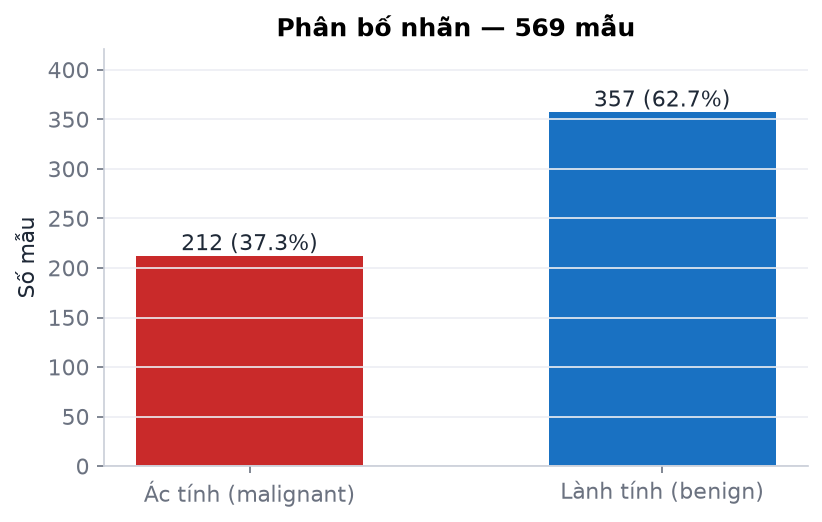
\includegraphics[width=0.6\textwidth]{01_phan_bo_nhan.png}
\caption{Phân bố nhãn trong \NSamples{} mẫu}
\end{figure}

Một phát hiện quan trọng khi thiết kế API: \NZeroFeatures{} đặc trưng \ZeroFeatures{} bằng \textbf{đúng 0} ở
\NZeroRows{} mẫu thật (khối u có đường viền không lõm). Vì vậy ràng buộc ``giá trị dương'' của schema chỉ áp dụng
cho 24 đặc trưng còn lại; sáu đặc trưng này chấp nhận giá trị 0. Nếu áp $> 0$ cho cả 30 trường, API sẽ từ chối
\NZeroRows{} mẫu hợp lệ.

\subsection{Trực quan hoá}

\begin{figure}[H]
\centering
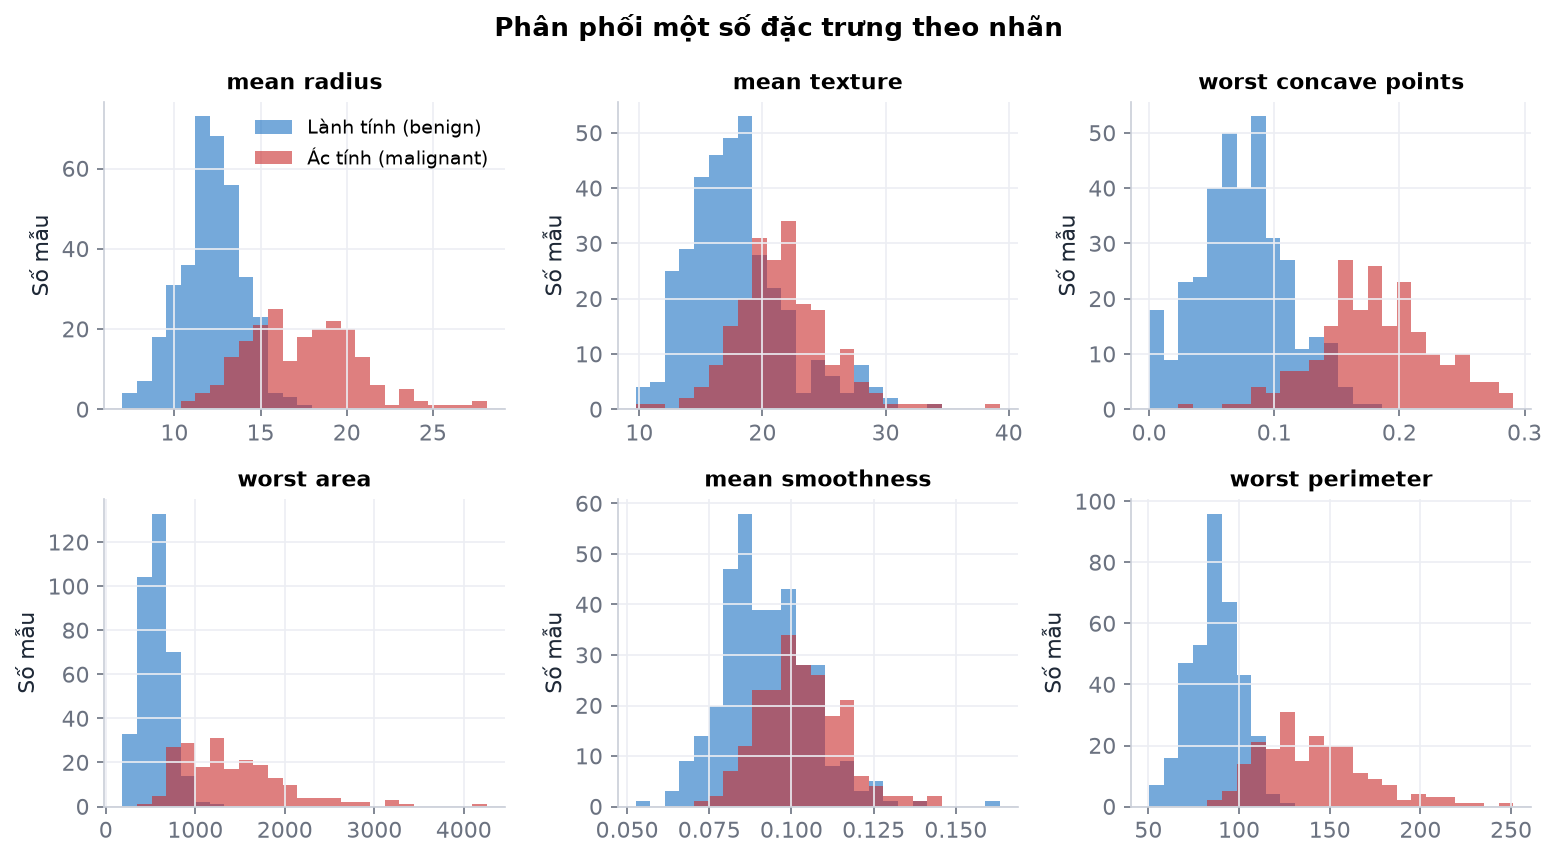
\includegraphics[width=\textwidth]{02_phan_phoi_dac_trung.png}
\caption{Phân phối sáu đặc trưng theo nhãn}
\label{fig:phan-phoi}
\end{figure}

Hình~\ref{fig:phan-phoi} cho thấy các đặc trưng về kích thước (\texttt{mean radius}, \texttt{worst area},
\texttt{worst perimeter}) và về hình dạng (\texttt{worst concave points}) tách hai lớp khá rõ: khối u ác tính có
nhân lớn hơn và đường viền lõm hơn. Ngược lại \texttt{mean smoothness} và \texttt{mean texture} chồng lấn nhiều ---
không đặc trưng đơn lẻ nào đủ để phân loại, nên cần mô hình kết hợp nhiều đặc trưng.

\begin{figure}[H]
\centering
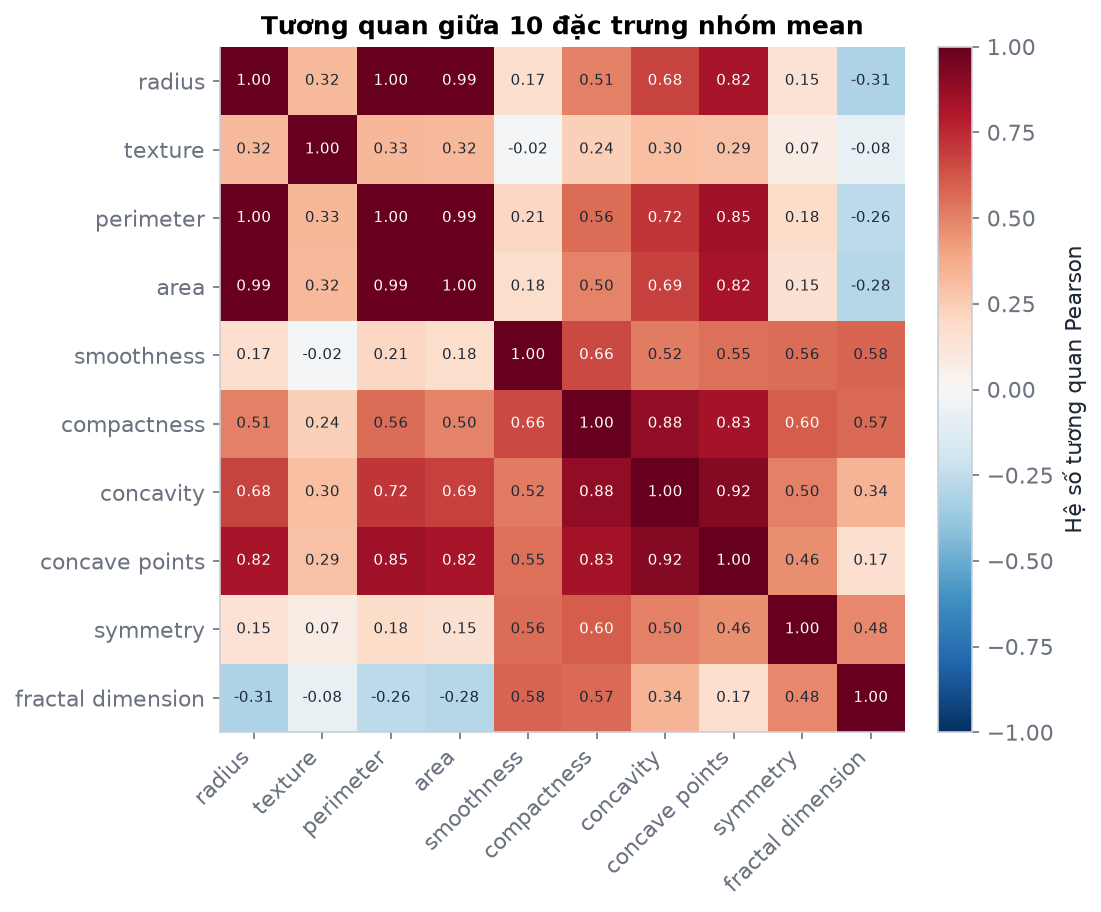
\includegraphics[width=0.78\textwidth]{03_tuong_quan.png}
\caption{Tương quan giữa mười đặc trưng nhóm \texttt{mean}}
\label{fig:tuong-quan}
\end{figure}

Radius, perimeter và area tương quan gần như tuyệt đối (hình~\ref{fig:tuong-quan}) --- đúng về mặt hình học, vì chu
vi và diện tích đều là hàm của bán kính. Concavity, concave points và compactness cũng tương quan mạnh. Dữ liệu vì
vậy dư thừa nhiều; kernel RBF trên đặc trưng đã chuẩn hoá xử lý được tình huống này mà không cần loại bớt đặc trưng.

\begin{figure}[H]
\centering
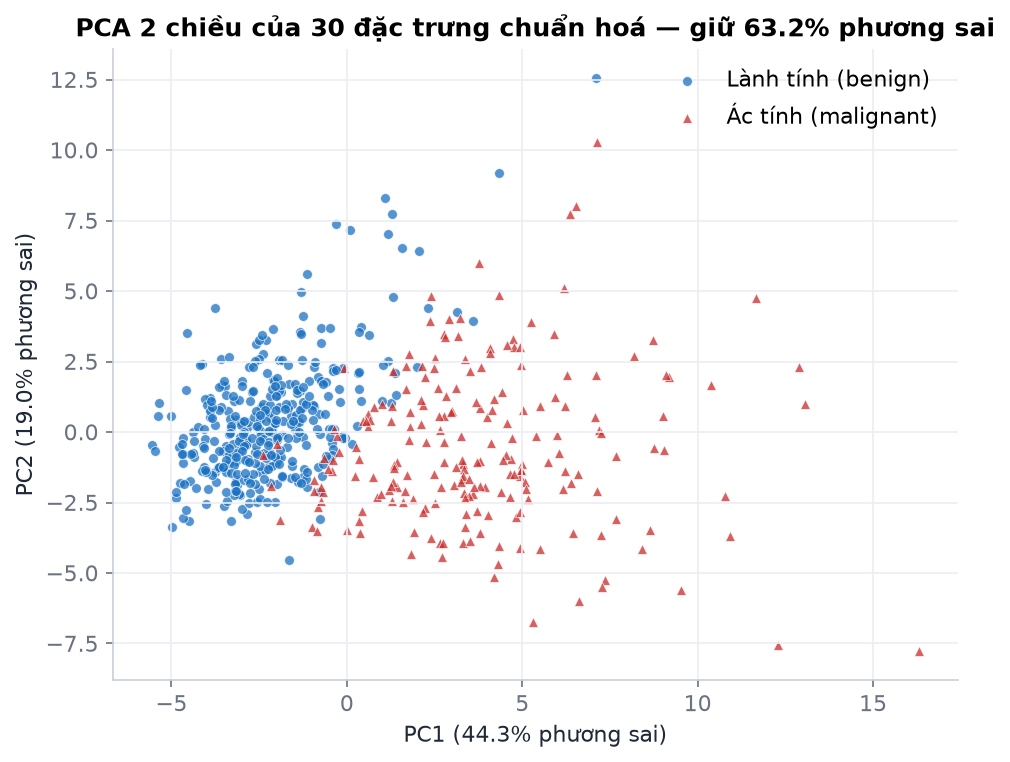
\includegraphics[width=0.72\textwidth]{04_pca.png}
\caption{Chiếu \NFeatures{} đặc trưng chuẩn hoá xuống hai thành phần chính}
\label{fig:pca}
\end{figure}

Hai thành phần chính đầu tiên giữ \PcaTotal{} phương sai (PC1 \PcaOne, PC2 \PcaTwo). Trên mặt phẳng này hai lớp đã
tách tương đối rõ theo PC1 nhưng vẫn có một vùng chồng lấn --- chính vùng này sinh ra các ca khó ở mục đánh giá.

% =============================================================================
\section{Huấn luyện mô hình SVM: quy trình và kiểm tra tính hiệu quả}
% =============================================================================

\subsection{Quy trình}
\begin{enumerate}
  \item \textbf{Chia dữ liệu}: 80\% huấn luyện (\NTrain{} mẫu), 20\% kiểm tra (\NTest{} mẫu: \TestMalignant{} ác tính,
        \TestBenign{} lành tính), \texttt{stratify=y}, \texttt{random\_state=\RandomState}.
  \item \textbf{Dò siêu tham số}: \texttt{GridSearchCV} với \texttt{StratifiedKFold(5)} \emph{chỉ trên tập huấn luyện}.
  \item \textbf{Hiệu chỉnh xác suất}: so sánh bốn cách bằng xác suất \emph{out-of-fold} trên tập huấn luyện.
  \item \textbf{Chọn ngưỡng}: trên chính các xác suất out-of-fold đó, rồi khoá lại.
  \item \textbf{Huấn luyện lại} trên toàn bộ tập huấn luyện và \textbf{đánh giá một lần duy nhất} trên tập kiểm tra.
  \item \textbf{Xuất artifact}: mô hình (\texttt{joblib}), \texttt{metadata.json} có phiên bản, mẫu test cho demo.
\end{enumerate}

Mọi lựa chọn (siêu tham số, cách hiệu chỉnh, ngưỡng) chỉ dùng tập huấn luyện. Tập kiểm tra được giữ kín cho tới
bước cuối, nên con số trên đó là ước lượng trung thực cho dữ liệu mới cùng phân phối.

\subsection{Dò siêu tham số}
Lưới gồm $C \in \{0{,}1;\ 1;\ 10;\ 100\}$ và $\gamma \in \{\texttt{scale};\ 0{,}001;\ 0{,}01;\ 0{,}1\}$ --- \GridConfigs{}
cấu hình, chấm bằng \GridScoring{} (trung bình recall của hai lớp, không để lớp đông át lớp ít). Toàn bộ lần tìm
kiếm mất \GridSeconds{} giây.

\begin{figure}[H]
\centering
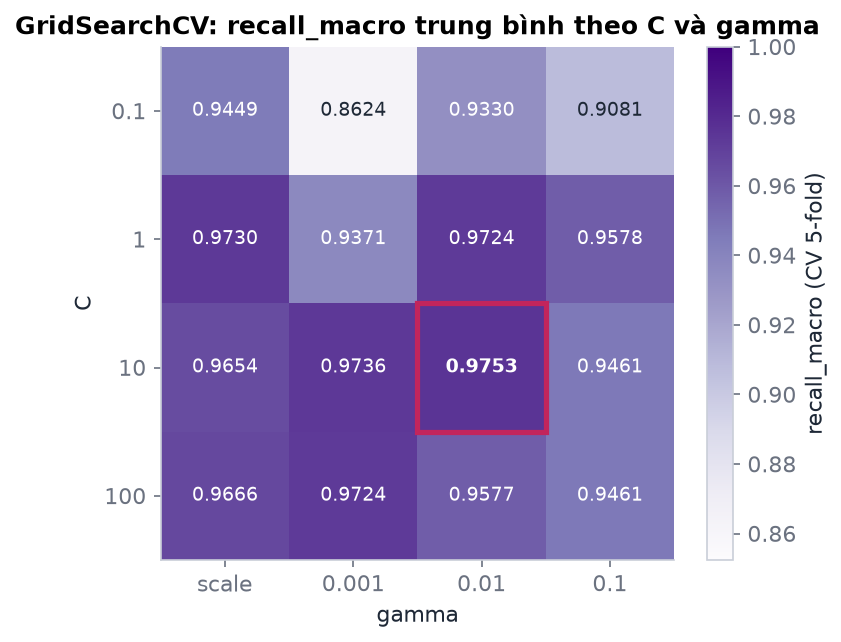
\includegraphics[width=0.7\textwidth]{05_grid_search.png}
\caption{recall\_macro trung bình qua 5 fold theo $C$ và $\gamma$ (ô viền đỏ là cấu hình được chọn)}
\label{fig:grid}
\end{figure}

Cấu hình tốt nhất là $C = \BestC$, $\gamma = \BestGamma$ với recall\_macro \GridCVMean{} $\pm$ \GridCVStd{}.
Hình~\ref{fig:grid} cho thấy $C = 0{,}1$ luôn kém (lề quá rộng, mô hình quá đơn giản), còn $\gamma = 0{,}1$ tụt ở
mọi $C$ (mỗi vector hỗ trợ ảnh hưởng vùng quá hẹp). Nhiều cấu hình ở vùng giữa cho điểm sát nhau, chênh lệch nhỏ
hơn độ lệch chuẩn giữa các fold --- mô hình không nhạy với lựa chọn chính xác trong vùng này.

\begin{table}[H]
\centering
\caption{Kết quả GridSearchCV, xếp theo thứ hạng}
\small
\begin{tabular}{@{}rrcr@{}}
\toprule
$C$ & $\gamma$ & recall\_macro (TB $\pm$ độ lệch) & Hạng \\
\midrule
\GridRows
\bottomrule
\end{tabular}
\end{table}

\subsection{Hiệu chỉnh xác suất}
Bốn cách lấy xác suất được so sánh trên xác suất \emph{out-of-fold} của tập huấn luyện (mỗi mẫu được dự đoán bởi
mô hình không nhìn thấy nó):

\begin{table}[H]
\centering
\caption{So sánh cách hiệu chỉnh xác suất (xác suất out-of-fold trên tập huấn luyện)}
\small
\begin{tabular}{@{}lrrrl@{}}
\toprule
Cách & Brier & Log-loss & ROC-AUC & Ghi chú \\
\midrule
\CalibRows
\bottomrule
\end{tabular}
\end{table}

\begin{figure}[H]
\centering
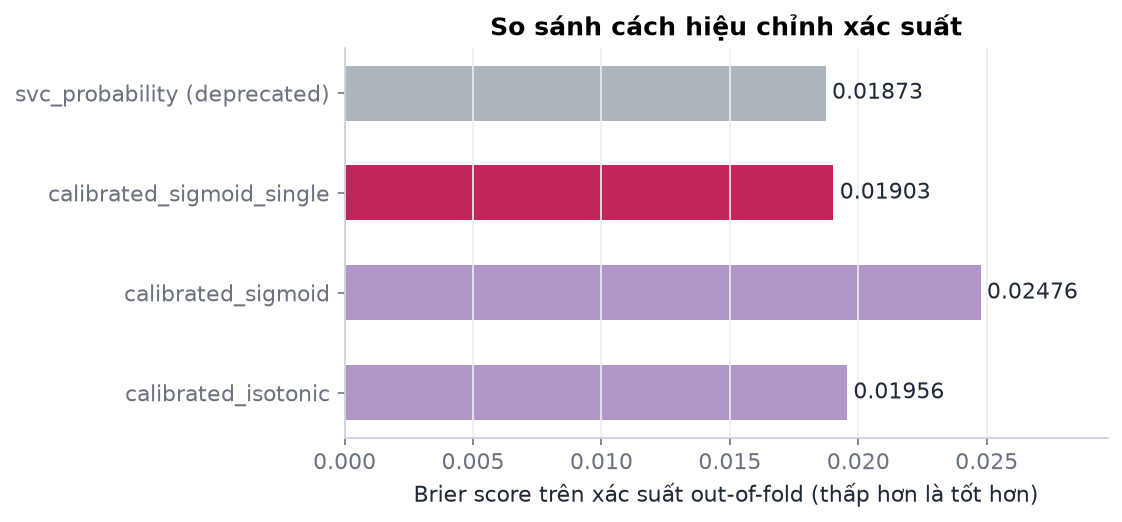
\includegraphics[width=0.8\textwidth]{06_hieu_chinh_xac_suat.png}
\caption{Brier score của bốn cách hiệu chỉnh (thấp hơn là tốt hơn)}
\end{figure}

\texttt{SVC(probability=True)} --- cách bài giảng dùng --- có Brier thấp nhất (\CalibBaselineBrier), nhưng tham số
này đã bị \textbf{deprecated từ scikit-learn 1.9 và sẽ bị xoá ở bản 1.11}; mô hình dùng nó sẽ không huấn luyện lại
được trên các phiên bản sau. Chính scikit-learn khuyên thay bằng
\texttt{CalibratedClassifierCV(SVC(), ensemble=False)}. Quy tắc chọn vì vậy là: \emph{Brier nhỏ nhất trong các cách
không bị deprecated}. Cách được chọn là \CalibChosen{} với Brier \CalibChosenBrier{} --- chỉ kém mốc tham chiếu ở
chữ số thập phân thứ tư. Isotonic (\CalibIsotonicBrier) có Brier gần tương đương nhưng log-loss cao hơn nhiều: với
vài trăm mẫu, hàm bậc thang cho ra các xác suất sát 0 hoặc 1 và bị phạt nặng khi sai.

\subsection{Chọn ngưỡng theo sensitivity}
\label{sec:nguong}
Quy tắc: chọn \emph{ngưỡng cao nhất} trên $P(\text{ác tính})$ mà sensitivity out-of-fold vẫn $\geq \TargetSens$
--- cao nhất để specificity lớn nhất có thể trong khi vẫn đạt mục tiêu. Ngưỡng được làm tròn \emph{xuống} bốn chữ số
thập phân để giá trị hiển thị trùng giá trị áp dụng (hạ ngưỡng chỉ có thể giữ nguyên hoặc tăng sensitivity).

\begin{figure}[H]
\centering
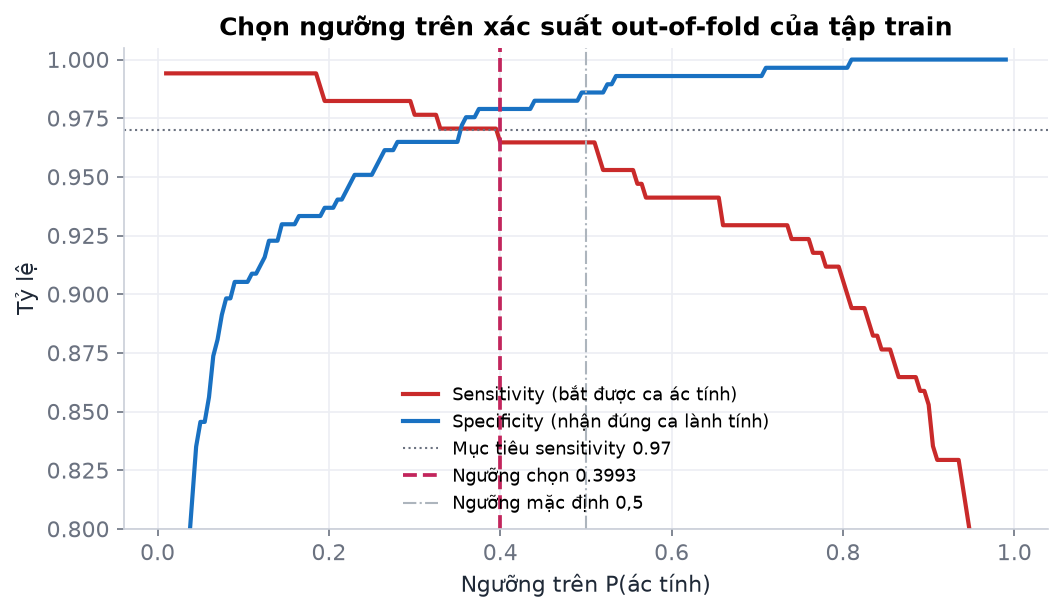
\includegraphics[width=0.85\textwidth]{07_chon_nguong.png}
\caption{Sensitivity và specificity out-of-fold theo ngưỡng; vạch đứt là ngưỡng được chọn}
\end{figure}

Kết quả: \textbf{ngưỡng $t = \Threshold$}. Trên dữ liệu out-of-fold, ngưỡng này bắt được \CVTP/\CVMalignant{} ca ác
tính (sensitivity \CVSens, specificity \CVSpec), trong khi ngưỡng mặc định $0{,}5$ chỉ bắt \CVHalfTP/\CVMalignant{}
(sensitivity \CVHalfSens{} --- dưới mục tiêu). Theo công thức ở mục 2, ngưỡng này tương đương coi việc bỏ sót một
ca ác tính đắt gấp khoảng \ImpliedCostRatio{} lần một lần báo động nhầm.

API luôn gán nhãn bằng \texttt{proba\_malignant >= threshold}, \emph{không} dùng \texttt{model.predict()}. Với
\texttt{SVC(probability=True)}, \texttt{predict} dựa trên dấu của điểm quyết định còn \texttt{predict\_proba} dựa
trên Platt scaling, nên hai kết quả có thể mâu thuẫn; dùng một quy tắc duy nhất bảo đảm nhãn và xác suất luôn
nhất quán.

\subsection{Các chỉ số đánh giá}
Lớp dương là \textbf{ác tính} (nhãn 0 trong scikit-learn, nên các hàm của scikit-learn cần \texttt{pos\_label=0}).
Với $TP, FN, FP, TN$ là số ca ác tính phát hiện đúng, ác tính bị bỏ sót, lành tính bị báo nhầm và lành tính
nhận đúng:
\[
  \text{Sensitivity} = \frac{TP}{TP + FN}, \quad
  \text{Specificity} = \frac{TN}{TN + FP}, \quad
  \text{Precision} = \frac{TP}{TP + FP}, \quad
  F_1 = \frac{2 \cdot \text{Precision} \cdot \text{Sensitivity}}{\text{Precision} + \text{Sensitivity}} .
\]
ROC-AUC là xác suất một ca ác tính ngẫu nhiên được chấm điểm cao hơn một ca lành tính ngẫu nhiên; PR-AUC
(average precision) tóm tắt đường precision--recall, nhạy hơn ROC-AUC khi lớp dương là thiểu số. Hai chỉ số này
đánh giá khả năng \emph{xếp hạng} qua mọi ngưỡng, còn bốn chỉ số trên đánh giá tại ngưỡng đã chọn.

\subsection{Kết quả}

\begin{table}[H]
\centering
\caption{Chỉ số tại ngưỡng đã khoá trên tập huấn luyện, kiểm định chéo và tập kiểm tra}
\label{tab:ket-qua}
\footnotesize
\setlength{\tabcolsep}{3.5pt}
\begin{tabular}{@{}lrrrrrrrrr@{}}
\toprule
Tập & Ngưỡng & Sens. & Spec. & Precision & F1 & ROC-AUC & PR-AUC & FN & FP \\
\midrule
\MetricRows
\bottomrule
\end{tabular}
\end{table}

Trên tập kiểm tra, mô hình đạt \textbf{sensitivity \TestSens} (bắt \TestTP/\TestMalignant{} ca ác tính),
\textbf{specificity \TestSpec}, precision ác tính \TestPrec, F1 \TestFOne, ROC-AUC \TestAUC{} và PR-AUC \TestPRAUC.
Brier score trên test là \TestBrier.

\paragraph{Kiểm tra quá khớp.} Sensitivity giảm từ \TrainSens{} (train) xuống \CVSens{} (CV) rồi \TestSens{} (test);
specificity từ \TrainSpec{} xuống \CVSpec{} rồi \TestSpec. Khoảng cách train--CV nhỏ, và test nằm trong vùng dao
động hợp lý của một tập chỉ có \TestMalignant{} ca ác tính: mô hình không quá khớp rõ rệt. Specificity trên test
thấp hơn CV --- xem phân tích lỗi bên dưới.

\begin{figure}[H]
\centering
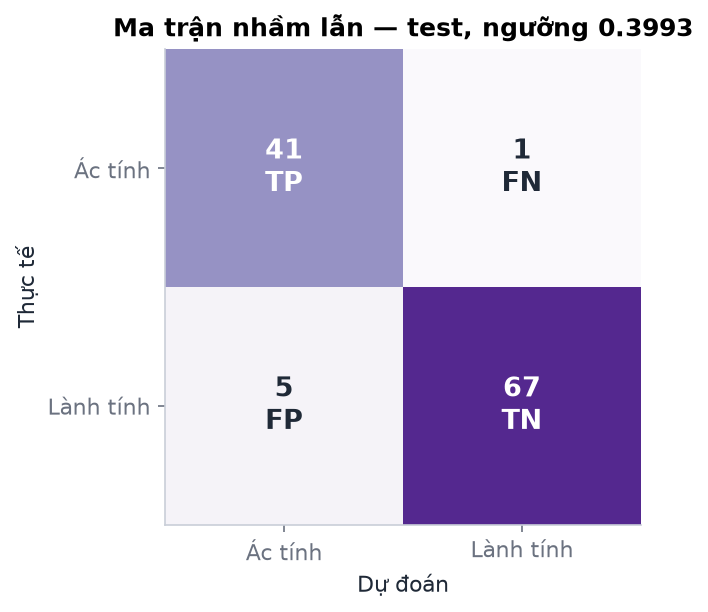
\includegraphics[width=0.5\textwidth]{08_ma_tran_nham_lan.png}
\caption{Ma trận nhầm lẫn trên tập kiểm tra tại ngưỡng \Threshold}
\end{figure}

\begin{figure}[H]
\centering
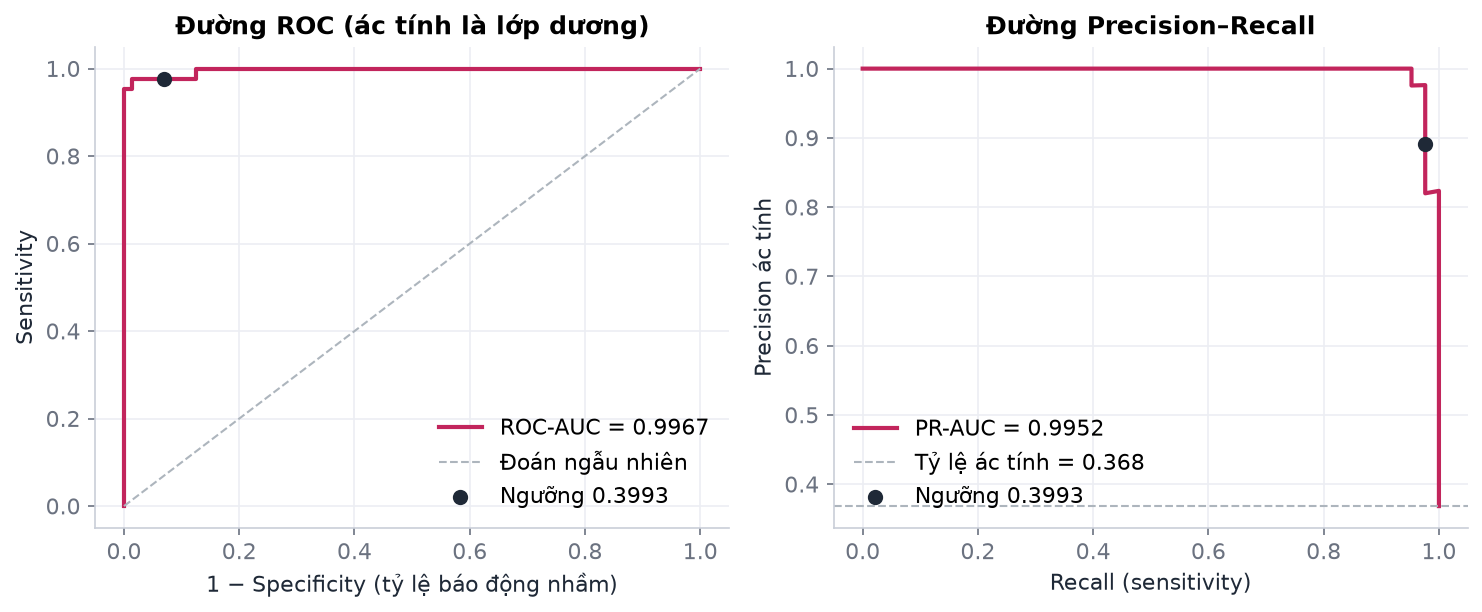
\includegraphics[width=\textwidth]{09_roc_pr.png}
\caption{Đường ROC và Precision--Recall trên tập kiểm tra; chấm đen là ngưỡng đã chọn}
\end{figure}

\begin{figure}[H]
\centering
\begin{minipage}{0.48\textwidth}\centering
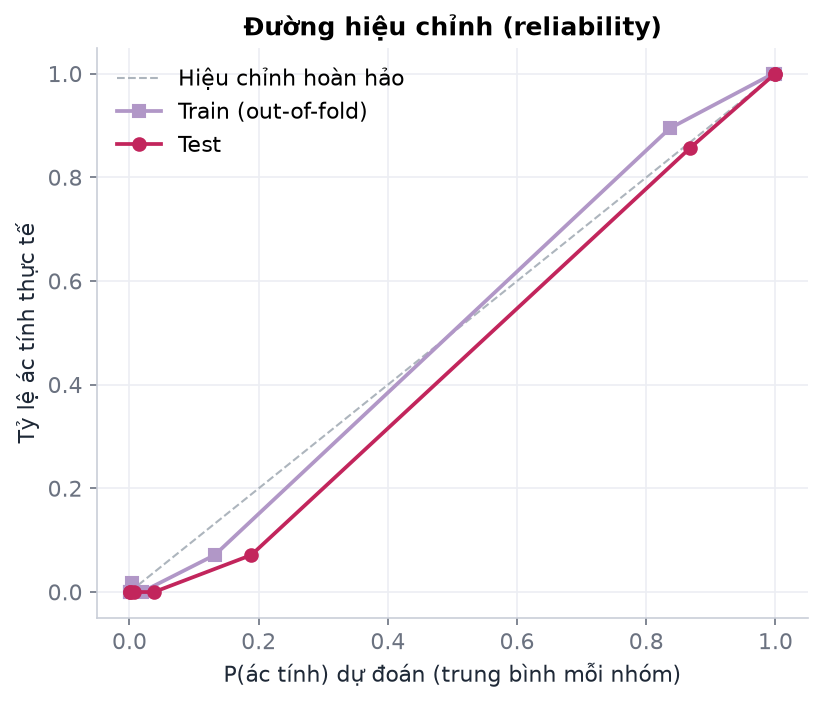
\includegraphics[width=\textwidth]{10_hieu_chinh.png}
\caption{Đường hiệu chỉnh xác suất}
\label{fig:reliability}
\end{minipage}\hfill
\begin{minipage}{0.5\textwidth}\centering
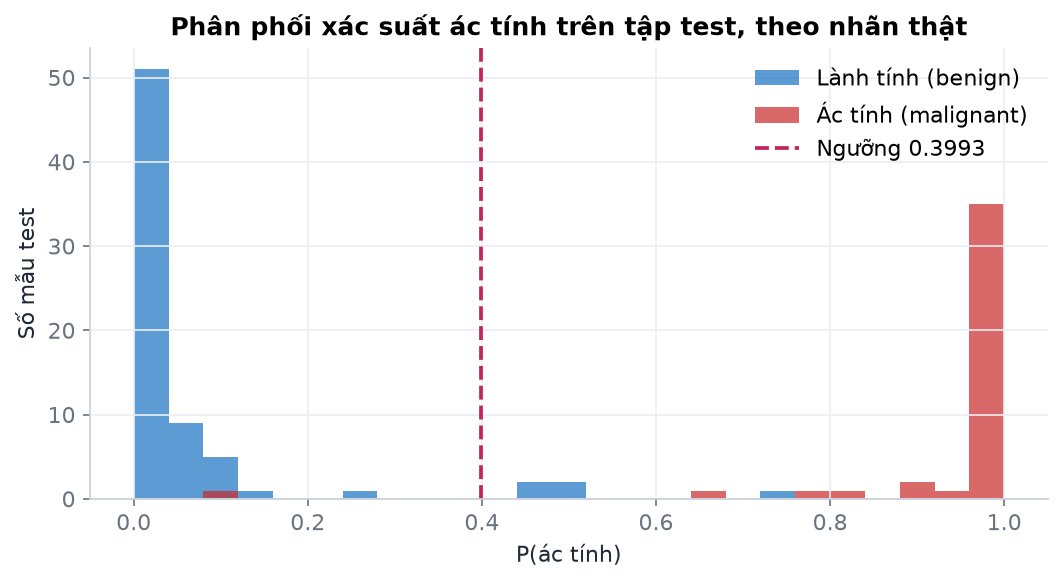
\includegraphics[width=\textwidth]{11_phan_phoi_xac_suat.png}
\caption{Phân phối $P(\text{ác tính})$ trên tập test}
\label{fig:phan-phoi-xs}
\end{minipage}
\end{figure}

Đường hiệu chỉnh (hình~\ref{fig:reliability}) bám sát đường chéo trên cả dữ liệu out-of-fold và tập test: xác suất
của mô hình phản ánh khá đúng tần suất ác tính thực tế. Hình~\ref{fig:phan-phoi-xs} cho thấy phần lớn mẫu được chấm
điểm gần 0 hoặc gần 1; các lỗi tập trung ở vùng giữa.

\subsection{Phân tích lỗi}

\begin{table}[H]
\centering
\caption{Các mẫu test bị dự đoán sai}
\small
\begin{tabular}{@{}rllr@{}}
\toprule
Chỉ số mẫu test & Nhãn thật & Dự đoán & $P(\text{ác tính})$ \\
\midrule
\ErrorRows
\bottomrule
\end{tabular}
\end{table}

Có \TestNErrors{} mẫu test bị dự đoán sai:
\begin{itemize}
  \item \textbf{\TestFN{} ca ác tính bị bỏ sót}, với $P(\text{ác tính}) = \MissedProba$. Xác suất này thấp hơn nhiều so
        với mọi ngưỡng hợp lý: ca này nằm sâu trong vùng lành tính của không gian đặc trưng, và muốn bắt được nó thì
        phải báo động nhầm phần lớn các ca lành tính. Đây là giới hạn của chính dữ liệu và mô hình, không phải của
        ngưỡng.
  \item \textbf{\TestFP{} ca lành tính bị báo nhầm} với $P(\text{ác tính})$ từ \FPMinProba{} đến \FPMaxProba; trong đó
        \FPBelowHalf{} ca có xác suất dưới $0{,}5$ --- tức là bị báo nhầm \emph{chỉ vì} ngưỡng đã được hạ.
\end{itemize}

\paragraph{Nhận xét trung thực về ngưỡng.} Trên riêng tập test này, ngưỡng mặc định $0{,}5$ cho \emph{cùng}
sensitivity (\HalfSens, \HalfFN{} ca bỏ sót) nhưng specificity cao hơn (\HalfSpec{}, \HalfFP{} ca báo nhầm so với
\TestFP). Nói cách khác, việc hạ ngưỡng đã trả giá bằng thêm báo động nhầm mà không bắt thêm ca ác tính nào \emph{trên
\TestMalignant{} ca test này}. Tuy vậy, ngưỡng không được chọn theo tập test --- làm thế là rò rỉ thông tin --- mà
theo dữ liệu kiểm định, nơi ngưỡng $0{,}5$ \emph{không đạt} mục tiêu (\CVHalfSens{} $<$ \TargetSens). Với số ca ác tính
nhỏ như vậy, chênh lệch một ca đã đổi sensitivity khoảng 2,4 điểm phần trăm; kết luận chắc chắn về ngưỡng cần tập
kiểm định lớn hơn, lý tưởng là dữ liệu ngoại bộ.

\subsection{Kiểm tra trước khi xuất mô hình}
Theo danh sách của bài giảng:
\begin{enumerate}
  \item So sánh train, cross-validation và test để nhận diện quá khớp --- bảng~\ref{tab:ket-qua}.
  \item Kiểm tra confusion matrix, đặc biệt false negative của lớp ác tính --- \TestFN{} ca trên tập test.
  \item Kiểm tra phân phối xác suất và hiệu chỉnh --- hình~\ref{fig:reliability} và~\ref{fig:phan-phoi-xs}.
  \item Thử dữ liệu nhập sai, thiếu trường, chuỗi thay số, NaN, vô cực --- bộ kiểm thử ở mục~\ref{sec:kiem-thu}.
  \item Ghi lại phiên bản dữ liệu (băm SHA-256 \texttt{\DataHashShort...}), thư viện (scikit-learn \SklearnVersion,
        numpy \NumpyVersion, Python \PythonVersion), seed (\RandomState) và siêu tham số --- trong \texttt{metadata.json}.
  \item Chỉ xuất artifact sau khi hoàn tất đánh giá độc lập.
\end{enumerate}

% =============================================================================
\section{Các công nghệ sử dụng để triển khai trực tuyến}
% =============================================================================

\begin{table}[H]
\centering
\caption{Công nghệ sử dụng}
\small
\begin{tabular}{@{}lp{0.68\textwidth}@{}}
\toprule
Thành phần & Vai trò \\
\midrule
scikit-learn \SklearnVersion & Pipeline, SVC, GridSearchCV, CalibratedClassifierCV, các chỉ số đánh giá \\
joblib & Lưu và nạp toàn bộ pipeline đã huấn luyện \\
FastAPI & Khung REST API: định tuyến, sinh tài liệu OpenAPI và Swagger UI tự động \\
Pydantic v2 & Khai báo và kiểm tra schema 30 trường đầu vào (kiểu, miền giá trị), sinh lỗi 422 \\
Uvicorn & Máy chủ ASGI chạy ứng dụng FastAPI \\
HTML / CSS / JavaScript & Bảng điều khiển web (SPA), không framework, gọi hai API bằng \texttt{fetch} \\
Chart.js, Lucide, Be Vietnam Pro & Biểu đồ, icon và font của giao diện --- tải sẵn trong dự án, không dùng CDN \\
SQLite & Cơ sở dữ liệu của API CSDL: tài khoản, lịch sử dự đoán, kết quả các lần train \\
bcrypt, PyJWT & Băm mật khẩu có muối; phát và xác minh token đăng nhập (HMAC-SHA256) \\
openpyxl & Xuất lịch sử và bảng so sánh mô hình ra tệp Excel \\
pytest, httpx, ruff & Kiểm thử tự động (TestClient) và kiểm tra phong cách mã \\
GitHub, GitHub Actions & Quản lý mã nguồn; CI chạy lint, kiểm thử, huấn luyện lại và smoke test mỗi lần push \\
Render & Nền tảng chạy dịch vụ web (gói Free), triển khai bằng Blueprint \texttt{render.yaml}, HTTPS sẵn có \\
matplotlib & Sinh hình cho tài liệu và slide (chỉ dùng khi phát triển) \\
\bottomrule
\end{tabular}
\end{table}

\paragraph{Vì sao FastAPI.} Khai báo schema bằng kiểu Python và Pydantic, FastAPI tự kiểm tra đầu vào, trả lỗi 422
có cấu trúc và sinh tài liệu tương tác tại \texttt{/docs} --- đúng những gì một API mô hình cần. Cơ chế
\texttt{lifespan} cho phép nạp mô hình \emph{một lần} khi khởi động.

\paragraph{Vì sao Render.} Render chạy trực tiếp ứng dụng Python từ kho GitHub, không cần Docker hay máy chủ riêng;
cấu hình triển khai lưu thành mã (\texttt{render.yaml}) nên dễ tái lập và review; có HTTPS và health check sẵn.
Gói Free đủ cho demo, đổi lại dịch vụ ngủ sau khoảng 15 phút không dùng.

% =============================================================================
\section{Chi tiết quy trình triển khai trực tuyến và vận hành}
% =============================================================================

\subsection{Cấu trúc kho mã nguồn}
\begin{lstlisting}[language={},numbers=none,caption={Cấu trúc thư mục}]
breast-cancer-svm/
|-- app/          API mo hinh: main.py, schemas.py, model_service.py, comparison.py,
|                 dashboard_api.py, classes.py, static/images (anh te bao hoc)
|-- db_api/       API CSDL: main.py, auth.py, history.py, runs.py, export.py, db.py, migrations/
|-- web/          module web: server.py, public/ (index.html, css, js, fonts, vendor)
|-- settings.py, security.py, seed.py
|-- artifacts/    breast_cancer_svm.joblib, metadata.json, test_samples.json
|-- scripts/      train.py, train_comparison.py, evaluate.py, make_sample_request.py, smoke_test.py
|-- tests/        test_api.py, test_model.py, test_auth.py, test_history.py, test_export.py,
|                 test_dashboard.py
|-- reports/      metrics.json, comparison.json, train_report.json, figures/
|-- docs/         latex/, model-card.md, kich-ban-demo.md, screenshots/
|-- .github/workflows/ci.yml
|-- requirements.txt, requirements-dev.txt, render.yaml, Makefile, tasks.ps1, .env.example
`-- README.md, CREDITS.md
\end{lstlisting}

\subsection{Artifact và metadata}
\texttt{artifacts/metadata.json} ghi mọi thông tin cần để phục vụ và truy vết mô hình: tên, phiên bản
(\ModelVersion), danh sách \NFeatures{} đặc trưng \emph{theo đúng thứ tự huấn luyện}, miền hợp lệ của từng đặc trưng,
ánh xạ nhãn, ngưỡng, cách hiệu chỉnh, siêu tham số, chỉ số trên test, ngày huấn luyện, băm dữ liệu, phiên bản thư
viện và câu cảnh báo. Khi khởi động, API kiểm tra danh sách đặc trưng trong metadata trùng với schema, và phiên bản
scikit-learn đang chạy trùng với lúc huấn luyện; sai lệch thì không nạp mô hình và \texttt{/health} trả 503.

\subsection{Hợp đồng API}

\begin{table}[H]
\centering
\caption{Các endpoint}
\small
\begin{tabular}{@{}llp{0.6\textwidth}@{}}
\toprule
Method & Đường dẫn & Chức năng \\
\midrule
GET  & \texttt{/} & Thông tin dịch vụ (JSON); trình duyệt được trả bảng điều khiển \\
GET  & \texttt{/health} & 200 khi mô hình đã nạp; 503 nếu artifact lỗi (Render dùng làm health check) \\
GET  & \texttt{/metadata} & Phiên bản, tên và miền của 30 đặc trưng, ánh xạ nhãn, ngưỡng, chỉ số test, cảnh báo \\
POST & \texttt{/predict} & Một bản ghi: 30 đặc trưng dạng phẳng hoặc \texttt{\{"features": \{...\}\}} \\
POST & \texttt{/predict/batch} & \texttt{\{"items": [...]\}}, từ 1 đến 100 bản ghi \\
GET  & \texttt{/samples} & Mẫu ngẫu nhiên từ tập \emph{kiểm tra} kèm nhãn thật (\texttt{n}, \texttt{label}, \texttt{seed}) \\
GET  & \texttt{/docs} & Swagger UI sinh tự động \\
GET  & \texttt{/ui} & Địa chỉ demo cũ, chuyển sang trang Chẩn đoán của bảng điều khiển \\
\bottomrule
\end{tabular}
\end{table}

Các endpoint phục vụ bảng điều khiển (lớp, thống kê, so sánh mô hình) và API cơ sở dữ liệu được trình bày ở
mục~\ref{sec:he-thong}.

Phản hồi của \texttt{/predict} gồm \texttt{predicted\_class}, \texttt{predicted\_label} (\texttt{malignant} /
\texttt{benign}), \texttt{predicted\_label\_vi}, \texttt{probability\_malignant}, \texttt{probability\_benign},
\texttt{threshold\_malignant}, \texttt{model\_version} và \texttt{warning}. API không nhận và không trả bất kỳ thông
tin định danh nào.

\paragraph{Kiểm tra đầu vào.} 30 trường được khai báo tường minh trong \texttt{app/schemas.py} (tên Python kèm
\emph{alias} đúng tên trong dataset, ví dụ \texttt{mean\_radius} $\leftrightarrow$ \texttt{"mean radius"}), ở chế độ
\emph{strict}. Các trường hợp bị từ chối với mã \textbf{422}:
\begin{itemize}
  \item thiếu hoặc thừa trường --- phản hồi kèm danh sách \texttt{missing} và \texttt{extra} như bài giảng;
  \item sai kiểu: chuỗi (kể cả \texttt{"12.5"}), \texttt{null}, mảng, object lồng nhau, \texttt{true}/\texttt{false};
  \item \texttt{NaN}, \texttt{Infinity}: bộ đọc JSON của Python chấp nhận các literal này, nên phải chặn tường minh;
  \item giá trị $\leq 0$ ở 24 đặc trưng luôn dương, giá trị âm ở \NZeroFeatures{} đặc trưng được phép bằng 0;
  \item giá trị vượt \UpperFactor{} lần mức lớn nhất quan sát được trong tập huấn luyện --- phản hồi kèm danh sách
        \texttt{out\_of\_range}.
\end{itemize}
Mã \textbf{503} khi mô hình chưa nạp được. Thông báo lỗi 422 không lặp lại dữ liệu đã gửi.

\subsection{Nhật ký và quyền riêng tư}
Middleware ghi cho mỗi request: mã request (\texttt{X-Request-ID}, sinh ngẫu nhiên nếu client không gửi), phương
thức, đường dẫn, mã trạng thái và độ trễ; endpoint dự đoán ghi thêm nhãn. \textbf{Không bao giờ} ghi giá trị xét
nghiệm --- có kiểm thử tự động bảo đảm điều này.

\begin{lstlisting}[language={},numbers=none,caption={Một dòng log khi dự đoán}]
INFO breast_cancer_api request_id=4bd29d4faca0 prediction=malignant
INFO breast_cancer_api request_id=4bd29d4faca0 method=POST path=/predict status=200 latency_ms=2.4
\end{lstlisting}

\subsection{Kiểm thử}
\label{sec:kiem-thu}
\texttt{tests/test\_api.py} hiện thực ma trận kiểm thử của bài giảng:
\begin{itemize}
  \item \textbf{Happy path}: đủ 30 trường số hữu hạn, cả hai dạng payload cho cùng kết quả; nhãn khớp quy tắc ngưỡng.
  \item \textbf{Thiếu / thừa trường}: 422 kèm tên trường; payload một trường của bài giảng liệt kê 29 trường thiếu.
  \item \textbf{Sai kiểu}: chuỗi, \texttt{null}, mảng, object, boolean.
  \item \textbf{Giá trị bất hợp lệ}: NaN, $\pm\infty$, 0 và âm ở đặc trưng dương, giá trị ngoài miền.
  \item \textbf{Khả dụng}: \texttt{/health}, 503 khi artifact lỗi, \texttt{X-Request-ID}.
  \item \textbf{Batch và samples}: giới hạn 1--100 bản ghi, lọc theo nhãn, tái lập bằng \texttt{seed}.
  \item \textbf{Quyền riêng tư}: giá trị gửi lên không xuất hiện trong log.
\end{itemize}
\texttt{tests/test\_model.py} là kiểm thử hồi quy của mô hình: băm dữ liệu trùng metadata, một số mẫu test cố định
phải trả đúng nhãn và xác suất đã ghi (kể cả ca bỏ sót và ca báo nhầm đã biết), chỉ số test trùng metadata và không
thấp hơn mức tối thiểu, sensitivity out-of-fold đạt mục tiêu.

Bốn tệp còn lại kiểm thử phần hệ thống (mục~\ref{sec:he-thong}): \texttt{test\_auth.py} (mật khẩu được băm bcrypt, trùng
tên, đăng nhập đúng/sai, token sai, tài khoản demo được seed, train lại cần đăng nhập), \texttt{test\_history.py} (lưu
và đọc lịch sử, mỗi người chỉ thấy và sửa được bản ghi của mình, nhãn thật, lọc theo mô hình),
\texttt{test\_export.py} (tệp Excel có header đậm màu, đúng các sheet, tên tệp có thời gian) và
\texttt{test\_dashboard.py} (ảnh có nguồn và tải được, thống kê theo lớp, PCA, bảng so sánh 5 mô hình, dòng SVM trong
bảng khớp metadata của mô hình triển khai, chuyển hướng từ địa chỉ demo cũ).

GitHub Actions (\texttt{.github/workflows/ci.yml}) chạy mỗi lần push: ruff, pytest trên artifact đã commit,
\emph{huấn luyện lại từ đầu} rồi pytest lần nữa (chứng minh artifact tái lập được), sinh hình và smoke test trên
máy chủ cục bộ.

\subsection{Cấu hình triển khai}
\lstinputlisting[language={},caption={render.yaml --- Render Blueprint}]{../../render.yaml}

Ba chi tiết dễ sai: đường dẫn ứng dụng \texttt{app.main:app} (gói \texttt{app}, tệp \texttt{main.py}, biến
\texttt{app}); \texttt{--host 0.0.0.0} để nhận kết nối từ ngoài container; \texttt{--port \$PORT} vì Render cấp cổng
động. Dịch vụ phục vụ đúng artifact đã commit, \emph{không} huấn luyện lại lúc build: con số trong tài liệu, slide và
API trực tuyến vì vậy là của cùng một mô hình. Phiên bản thư viện khoá trong \texttt{requirements.txt} và
\texttt{PYTHON\_VERSION} trong \texttt{render.yaml}. Biến \texttt{SERVICE\_MODE=single} cho một tiến trình chạy cả ba
module; \texttt{JWT\_SECRET} do Render tự sinh một lần và không bao giờ nằm trong mã nguồn.

\subsection{Các bước triển khai}
\begin{enumerate}
  \item Tạo repository trên GitHub, đẩy mã lên nhánh \texttt{main} (thư mục \texttt{artifacts/} phải được commit).
  \item Trên Render chọn \textbf{New} $\rightarrow$ \textbf{Blueprint}, kết nối repository; Render đọc
        \texttt{render.yaml} và hiển thị trước dịch vụ sẽ tạo.
  \item Chọn \textbf{Apply}, theo dõi build log (\texttt{pip install -r requirements.txt}) và runtime log cho tới khi
        health check \texttt{/health} thành công.
  \item Truy cập \url{https://breast-cancer-svm-api-f2qq.onrender.com}, kiểm tra \texttt{/health}, \texttt{/docs},
        \texttt{/metadata}, \texttt{/predict}.
  \item Chạy \texttt{python scripts/smoke\_test.py <URL>}.
\end{enumerate}
Cách thủ công (\textbf{New} $\rightarrow$ \textbf{Web Service}) cũng được: build command
\texttt{pip install -r requirements.txt}, start command
\texttt{uvicorn app.main:app --host 0.0.0.0 --port \$PORT}, thêm biến môi trường \texttt{PYTHON\_VERSION}.

\subsection{Kiểm tra sau triển khai}
\texttt{scripts/smoke\_test.py} (chỉ dùng thư viện chuẩn) thực hiện bảy bước kiểm tra của bài giảng trên một URL bất kỳ:
\begin{enumerate}
  \item \textbf{Smoke}: \texttt{GET /health} trả 200 (chờ tối đa 2 phút cho dịch vụ đang ngủ thức dậy).
  \item \textbf{Schema}: \texttt{/docs} hiển thị, OpenAPI có đủ 30 trường.
  \item \textbf{Prediction}: gửi \texttt{sample\_request.json} --- đúng payload đã dùng ở máy.
  \item \textbf{Negative}: thiếu một trường phải trả 422 và nêu đúng tên trường.
  \item \textbf{Log}: lỗi không lặp lại payload, có \texttt{X-Request-ID}; đọc thêm Logs trên Render.
  \item \textbf{Version}: \texttt{model\_version} thống nhất giữa \texttt{/health}, \texttt{/predict}, \texttt{/metadata}.
  \item \textbf{Restart}: artifact đang phục vụ trùng bản đã commit (băm dữ liệu, ngày huấn luyện); khởi động lại
        dịch vụ trên Render rồi chạy lại script.
\end{enumerate}

\subsection{Bảo mật và giám sát}
\paragraph{Bảo mật.} HTTPS do Render cung cấp; API không thu thập dữ liệu định danh; log không chứa payload; giới
hạn kích thước batch (100 bản ghi); không có secret nào trong mã nguồn. Mật khẩu chỉ lưu dạng băm bcrypt, token JWT
có hạn dùng, mọi truy vấn lịch sử đều lọc theo \texttt{user\_id} của token; API CSDL chỉ nhận request từ trang web
(CORS). Lịch sử lưu 30 số đo mà chính người dùng đã gửi --- không có trường nào cho tên hay mã bệnh nhân. Nếu API không hoàn toàn công khai cần thêm
xác thực, rate limit và timeout ở lớp gateway, quy định thời gian lưu và quy trình xoá dữ liệu, quét phụ thuộc định kỳ.

\paragraph{Giám sát.} Theo dõi tỷ lệ lỗi HTTP, độ trễ, số request và trạng thái health check (log có sẵn các trường
này); theo dõi phân phối đặc trưng và tần suất lỗi 422 \texttt{out\_of\_range} để phát hiện trôi dữ liệu; theo dõi
tỷ lệ nhãn dự đoán và mức độ tự tin. Khi có nhãn thật: đánh giá lại sensitivity, specificity, hiệu chỉnh và sai lệch
theo nhóm; duy trì phiên bản mô hình, khả năng rollback và quy trình phê duyệt mô hình mới.

\subsection{Các lỗi thường gặp}
\begin{itemize}
  \item \texttt{ModuleNotFoundError}: thiếu thư viện trong \texttt{requirements.txt}.
  \item \texttt{/health} trả 503 ``Artifact huấn luyện bằng scikit-learn \dots'': phiên bản trên Render khác lúc
        huấn luyện --- kiểm tra \texttt{requirements.txt} và \texttt{PYTHON\_VERSION}.
  \item \texttt{FileNotFoundError} cho \texttt{.joblib}: quên commit thư mục \texttt{artifacts/}.
  \item \texttt{Error loading ASGI app}: sai đường dẫn \texttt{app.main:app}.
  \item Dịch vụ treo ở \emph{Deploying}: đặt cứng cổng hoặc dùng \texttt{127.0.0.1} thay vì \texttt{0.0.0.0}.
  \item \texttt{422 Unprocessable Entity}: payload sai --- đọc \texttt{missing}, \texttt{extra}, \texttt{out\_of\_range}.
  \item Request đầu tiên rất chậm: dịch vụ Free đang ngủ, chờ 30--60 giây.
\end{itemize}

% =============================================================================
\section{Bảng điều khiển, tài khoản và so sánh mô hình}
\label{sec:he-thong}
% =============================================================================

Ngoài API chẩn đoán theo bài giảng, sản phẩm được xây thành một hệ thống hoàn chỉnh theo cùng kiến trúc với dự án
da1: giao diện bảng điều khiển, tài khoản người dùng, lịch sử dự đoán trong cơ sở dữ liệu, so sánh năm mô hình phân
loại và xuất Excel. API \texttt{/predict} và các endpoint ở mục trên giữ nguyên --- phần này chỉ \emph{thêm}.

\subsection{Kiến trúc ba module}

\begin{table}[H]
\centering
\caption{Ba module của hệ thống}
\small
\begin{tabular}{@{}lllp{0.46\textwidth}@{}}
\toprule
Module & Mã nguồn & Cổng & Trách nhiệm \\
\midrule
Web & \texttt{web/} & 8080 & Giao diện; chỉ gọi hai API qua HTTP, không nạp mô hình, không mở CSDL \\
API mô hình & \texttt{app/} & 8000 & Chẩn đoán SVM, so sánh 5 mô hình, thống kê dữ liệu, ảnh minh hoạ \\
API CSDL & \texttt{db\_api/} & 8001 & Đăng ký/đăng nhập, lịch sử dự đoán, kết quả các lần train, xuất Excel \\
\bottomrule
\end{tabular}
\end{table}

Hai API không gọi nhau: trang web \emph{điều phối} --- gọi API mô hình để dự đoán hoặc train lại, rồi gửi kết quả sang
API CSDL kèm token. API mô hình chỉ \emph{xác minh} token (dùng chung \texttt{JWT\_SECRET}) để khoá chức năng train lại.
Hệ thống chạy được theo hai cách: \textbf{tách} ba tiến trình trên ba cổng (\texttt{tasks.ps1 run-split}) khi chạy ở
máy, hoặc \textbf{gộp} (\texttt{SERVICE\_MODE=single}) trên gói Free của Render --- \texttt{uvicorn app.main:app} gắn API
CSDL tại \texttt{/db} và phục vụ thư mục web tại \texttt{/}; mã của ba module vẫn tách riêng.

\subsection{Tài khoản, lịch sử và cơ sở dữ liệu}
API CSDL dùng SQLite, lược đồ tạo bằng các tệp migration đánh số trong \texttt{db\_api/migrations/} (mỗi tệp chạy một lần,
ghi vào bảng \texttt{schema\_migrations}).

\begin{table}[H]
\centering
\caption{Các bảng của cơ sở dữ liệu}
\small
\begin{tabular}{@{}lp{0.72\textwidth}@{}}
\toprule
Bảng & Nội dung \\
\midrule
\texttt{users} & tên đăng nhập (không phân biệt hoa thường), mật khẩu băm bcrypt, thời điểm tạo \\
\texttt{predictions} & \texttt{user\_id}, thời điểm (UTC), mô hình, 30 số đo (JSON), nhãn dự đoán, $P(\text{ác tính})$,
                       ngưỡng, nhãn thật (nếu có), mã mẫu test, thời gian chạy \\
\texttt{training\_runs} & mỗi lần train: người train, thời điểm, số mẫu train/test, mục tiêu sensitivity, mô hình tốt nhất \\
\texttt{model\_runs} & bảng đánh giá 5 mô hình của mỗi lần train: sensitivity, specificity, precision, F1, ROC-AUC, PR-AUC,
                       Brier, ngưỡng, FN, FP, CV, thời gian, tham số tốt nhất \\
\bottomrule
\end{tabular}
\end{table}

Mật khẩu được băm bằng \textbf{bcrypt} có muối ngẫu nhiên; đăng nhập trả về \textbf{JWT} ký HMAC-SHA256 có hạn dùng. Truy
vấn lịch sử luôn kèm \texttt{user\_id} của token, nên mỗi người chỉ thấy và sửa được bản ghi của mình. Khi lưu một dự
đoán làm từ mẫu test, nhãn thật được ghi kèm để lịch sử cho biết đúng hay sai; người dùng cũng có thể ghi nhãn thật đã
xác nhận cho bản ghi nhập tay. \textbf{Xuất Excel} (openpyxl) cho hai loại dữ liệu: lịch sử (theo bộ lọc ngày và mô hình;
một sheet dự đoán, một sheet 30 số đo, một sheet bộ lọc) và bảng so sánh mô hình (lần train mới nhất kèm lịch sử mọi lần
train); hàng tiêu đề in đậm nền tím, cột tự giãn, tên tệp có thời gian. Ổ đĩa gói Free của Render không bền nên SQLite
được tạo lại mỗi lần khởi động; \texttt{seed.py} tạo lại tài khoản dùng thử \texttt{demo} / \texttt{demo123} và lần so
sánh đầu tiên.

\subsection{So sánh năm mô hình phân loại}
Năm mô hình --- SVM kernel RBF (mô hình triển khai), SVM tuyến tính, Logistic Regression, K láng giềng gần và Random Forest
--- đi qua \emph{đúng quy trình} của mô hình chính: \texttt{GridSearchCV} với \texttt{StratifiedKFold(5)} chấm bằng
\texttt{recall\_macro} chỉ trên tập train; xác suất (hai mô hình SVM bọc trong \texttt{CalibratedClassifierCV}); ngưỡng
riêng cho mỗi mô hình chọn trên xác suất out-of-fold để sensitivity $\geq \TargetSens$; đánh giá một lần trên tập test; đo
thời gian train và thời gian dự đoán (trung bình mỗi mẫu qua 200 lần dự đoán cả tập test) bằng \texttt{time.perf\_counter}.
Toàn bộ quy trình cho cả năm mô hình mất khoảng \CmpSeconds{} giây.

\begin{table}[H]
\centering
\caption{So sánh năm mô hình trên tập kiểm tra, mỗi mô hình ở ngưỡng riêng (dòng in đậm: CV cao nhất)}
\label{tab:so-sanh}
\footnotesize
\setlength{\tabcolsep}{3.5pt}
\begin{tabular}{@{}lrrrrrrrr@{}}
\toprule
Mô hình & CV & Sens. & Spec. & ROC-AUC & Ngưỡng & FN/FP & Train (ms) & Predict ($\mu$s) \\
\midrule
\CmpRows
\bottomrule
\end{tabular}
\end{table}

Ba nhận xét:
\begin{itemize}
  \item \CmpBestLabel{} có CV recall\_macro cao nhất (\CmpBestCV{} $\pm$ \CmpBestCVStd), nhưng chỉ hơn SVM RBF
        (\CmpSvmCV{} $\pm$ \CmpSvmCVStd) \CmpGap{} --- nhỏ hơn nhiều so với độ lệch giữa các fold. Trên dữ liệu này các
        mô hình tốt tương đương nhau; sản phẩm vẫn triển khai SVM theo yêu cầu đề bài, và bảng so sánh được trình bày
        đúng như kết quả đo được.
  \item Ở cùng mục tiêu sensitivity, các mô hình khác nhau chủ yếu ở \emph{specificity} --- số ca báo nhầm phải trả để
        giữ sensitivity cao. Đây là chỉ số nên nhìn khi so sánh mô hình sàng lọc.
  \item Về tốc độ, \CmpFastestLabel{} dự đoán nhanh nhất (\CmpFastestUs{} $\mu$s mỗi mẫu). Giao diện gắn nhãn
        \emph{Nhanh} (không quá \CmpSpeedFast{} lần mô hình nhanh nhất), \emph{Trung bình} (không quá \CmpSpeedMedium{}
        lần) hoặc \emph{Chậm}. Với dữ liệu nhỏ, mọi thời gian chỉ tính bằng mili giây và dao động giữa các lần chạy; chỉ
        thứ tự tương đối là đáng tin.
\end{itemize}
Người dùng đã đăng nhập có thể bấm \emph{Train lại} trên giao diện: API mô hình chạy lại toàn bộ quy trình, trang web lưu
bảng kết quả vào \texttt{training\_runs} và \texttt{model\_runs}.

\subsection{Giao diện bảng điều khiển}
Giao diện tông tím lavender: thanh bên có ảnh thu nhỏ của hai loại khối u, thẻ trắng bo góc, biểu đồ vẽ bằng Chart.js.
Font (Be Vietnam Pro), thư viện biểu đồ và bộ icon (Lucide) nằm trong dự án, không tải từ CDN. Mọi con số trên giao diện
lấy từ API. Mỗi khối có trạng thái đang tải, rỗng và lỗi; dưới 1024\,px bố cục chuyển thành một cột và thanh bên thành
dãy tab ngang.

\paragraph{Hình ảnh.} Hai ảnh tế bào học là phết chọc hút kim nhỏ nhuộm Papanicolaou --- cùng loại mẫu mà bộ dữ liệu
đo đặc trưng: u xơ tuyến vú (lành tính) và ung thư biểu mô ống tuyến vú (ác tính), tác giả Nephron, giấy phép
CC BY-SA 3.0, từ Wikimedia Commons. Ảnh được tải về dự án (không liên kết trực tiếp); dưới mỗi ảnh lớn có chú thích
``Nguồn: tác giả, giấy phép, liên kết''. Tệp \texttt{CREDITS.md} liệt kê nguồn của ảnh, icon, font, thư viện và dữ liệu.

\begin{figure}[H]
\centering
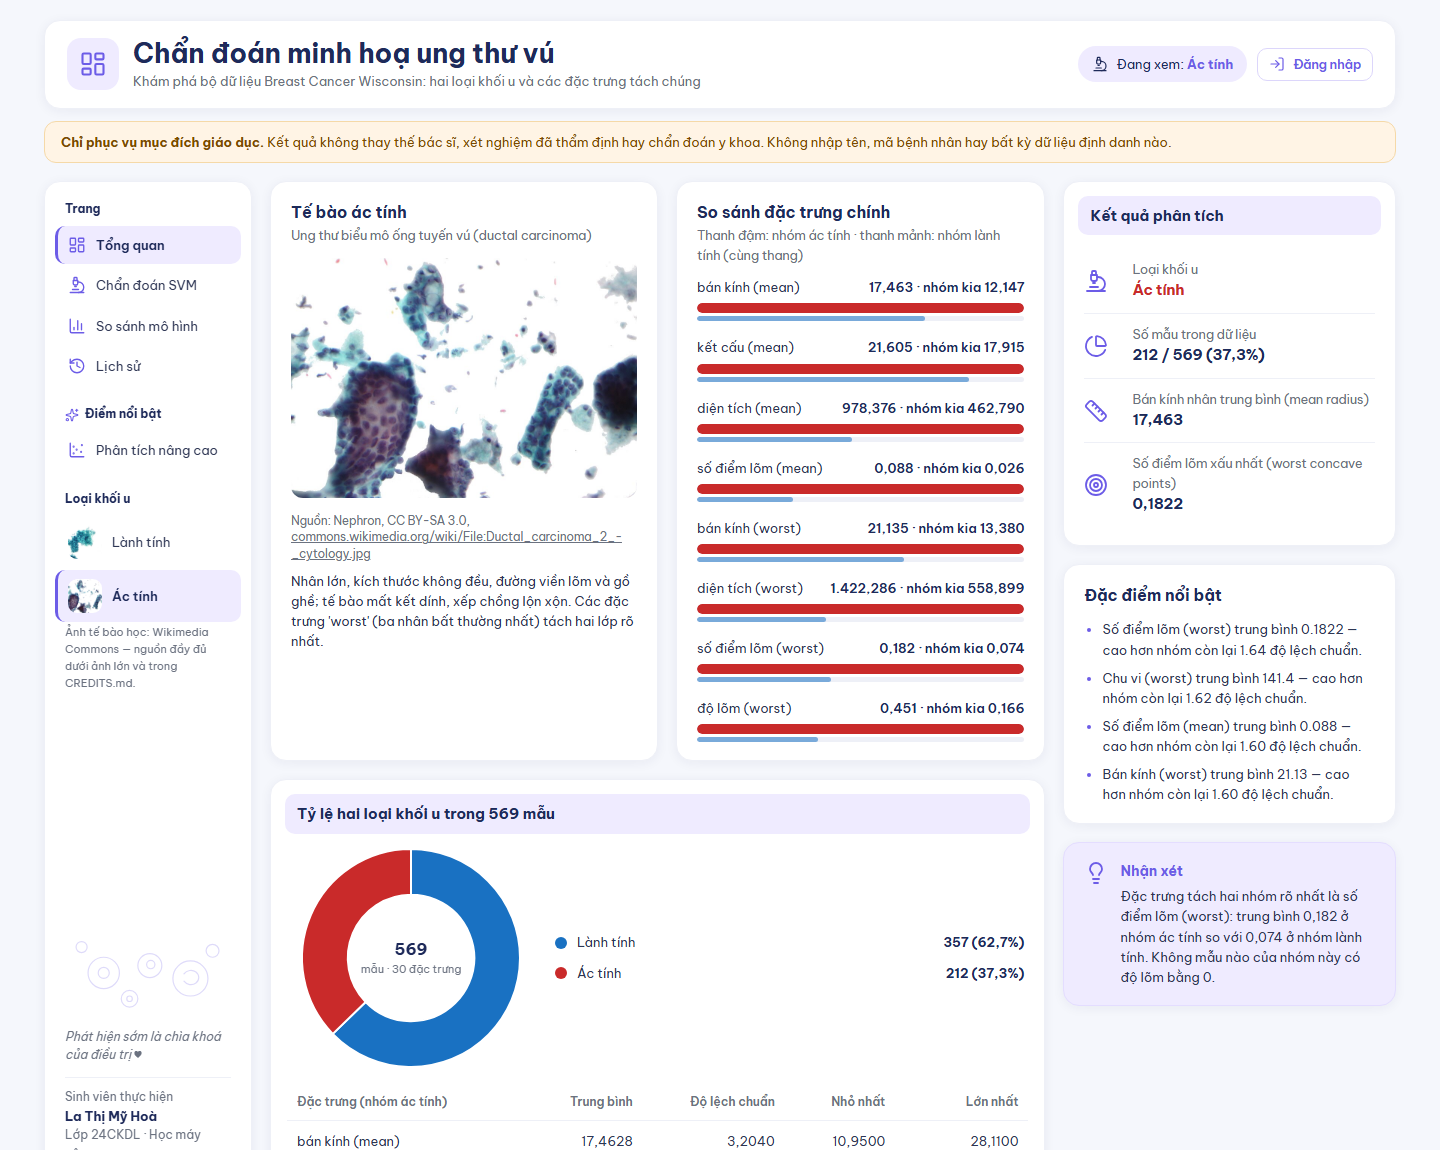
\includegraphics[width=\textwidth]{web_tong_quan.png}
\caption{Trang Tổng quan: ảnh tế bào học, so sánh đặc trưng giữa hai nhóm, tỷ lệ lớp, đặc điểm nổi bật và nhận xét}
\end{figure}

\begin{figure}[H]
\centering
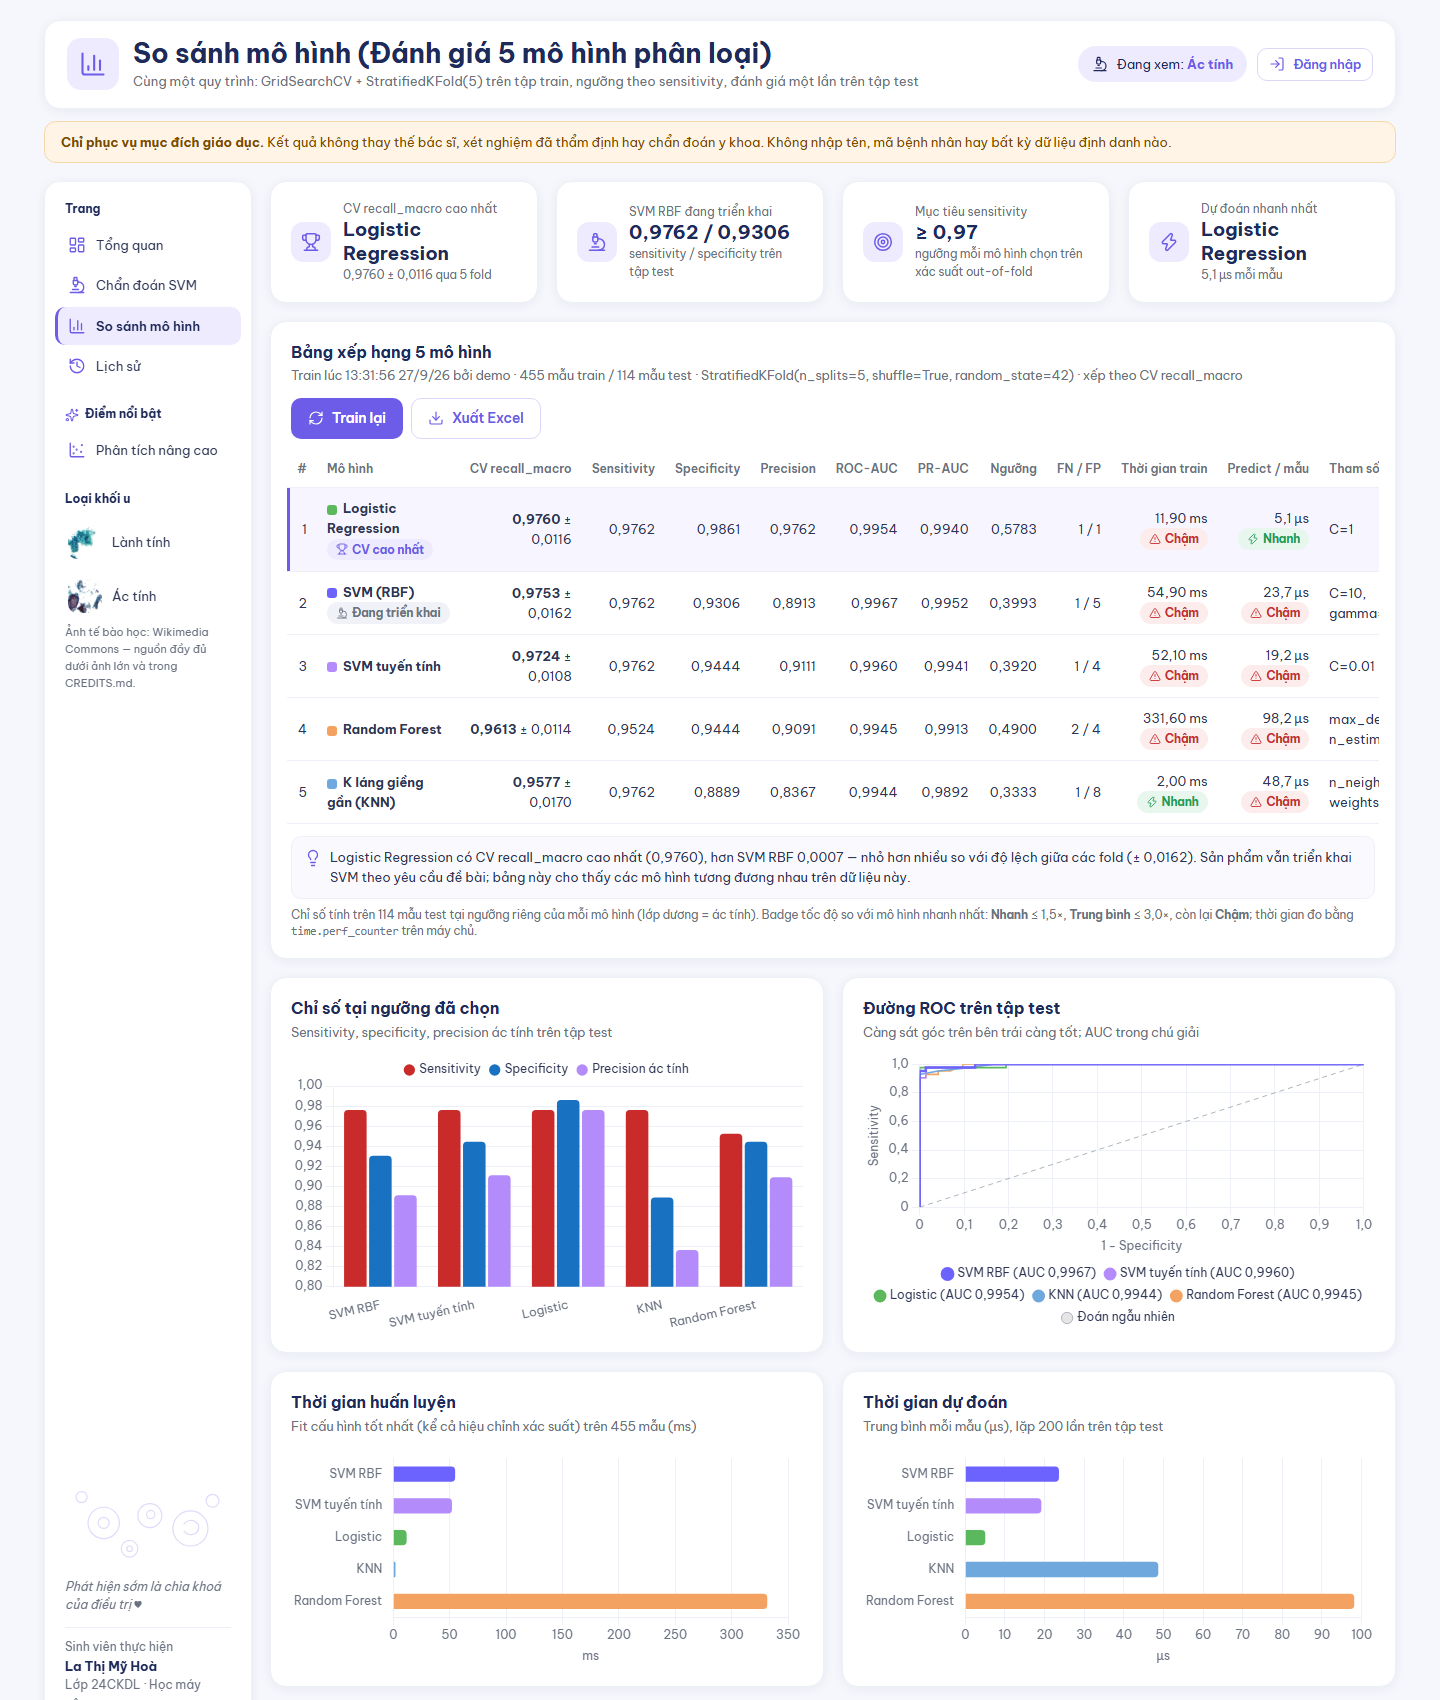
\includegraphics[width=\textwidth]{web_so_sanh.png}
\caption{Trang So sánh mô hình: bảng xếp hạng, badge tốc độ, chỉ số tại ngưỡng, đường ROC và thời gian}
\end{figure}

\paragraph{Điểm nổi bật --- khám phá ngưỡng quyết định.} Trang \emph{Phân tích nâng cao} cho kéo một thanh trượt ngưỡng
trên $P(\text{ác tính})$ của 114 mẫu test: ma trận nhầm lẫn, sensitivity, specificity, precision, số ca bỏ sót và báo
nhầm, histogram xác suất theo nhãn thật (có vạch ngưỡng) và điểm vận hành trên đường ROC đều thay đổi tức thì; câu nhận
xét so sánh với ngưỡng đã khoá. Công cụ này biến phần lý thuyết ở mục~\ref{sec:nguong} thành thứ người xem tự thử được,
đồng thời nhắc rằng chọn lại ngưỡng theo tập test là rò rỉ thông tin. Trang có thêm biểu đồ PCA 2D của toàn bộ dữ liệu.

\begin{figure}[H]
\centering
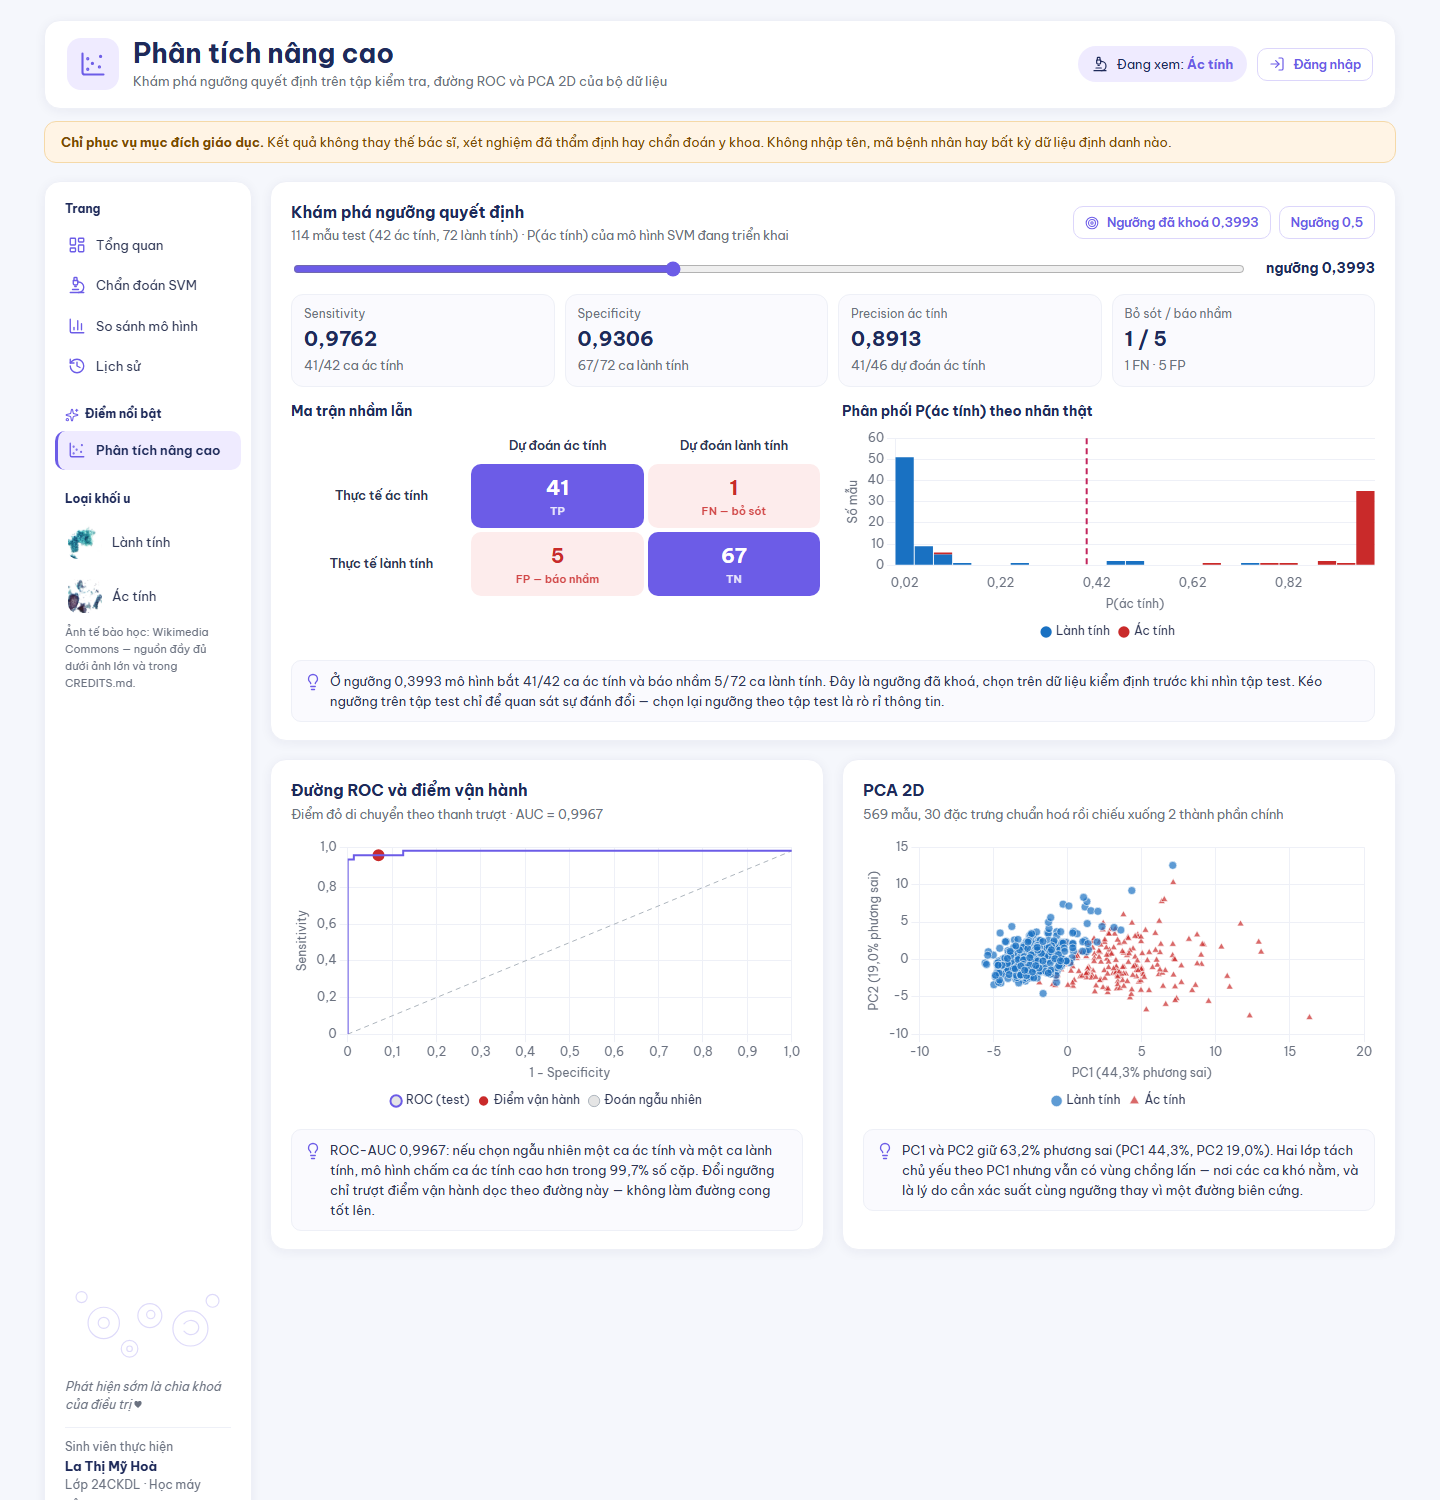
\includegraphics[width=\textwidth]{web_phan_tich.png}
\caption{Trang Phân tích nâng cao: khám phá ngưỡng, đường ROC với điểm vận hành, PCA 2D}
\end{figure}

\subsection{Các endpoint bổ sung}

\begin{table}[H]
\centering
\caption{Endpoint bổ sung của API mô hình}
\small
\begin{tabular}{@{}llp{0.55\textwidth}@{}}
\toprule
Method & Đường dẫn & Chức năng \\
\midrule
GET  & \texttt{/classes} & Hai loại khối u: mô tả, ảnh, tác giả, giấy phép, nguồn \\
GET  & \texttt{/dataset/summary} & Thống kê 30 đặc trưng theo lớp, các đặc trưng tách lớp rõ nhất \\
GET  & \texttt{/dataset/pca} & PCA 2D của 569 mẫu chuẩn hoá \\
GET  & \texttt{/models/metrics} & Bảng so sánh 5 mô hình \\
POST & \texttt{/models/train} & Train lại 5 mô hình (cần JWT) \\
GET  & \texttt{/analysis/test-scores} & Nhãn thật và $P(\text{ác tính})$ của 114 mẫu test \\
\bottomrule
\end{tabular}
\end{table}

\begin{table}[H]
\centering
\caption{Endpoint của API CSDL (trên Render có tiền tố \texttt{/db})}
\small
\begin{tabular}{@{}llp{0.52\textwidth}@{}}
\toprule
Method & Đường dẫn & Chức năng \\
\midrule
POST  & \texttt{/auth/register}, \texttt{/auth/login} & Đăng ký, đăng nhập; trả về JWT \\
GET   & \texttt{/auth/me} & Thông tin tài khoản \\
POST  & \texttt{/predictions} & Lưu một hoặc nhiều dự đoán \\
GET   & \texttt{/predictions} & Lịch sử của chính người dùng, lọc ngày và mô hình, phân trang \\
PATCH & \texttt{/predictions/\{id\}} & Ghi nhãn thật đã xác nhận \\
POST  & \texttt{/model-runs} & Lưu bảng đánh giá của một lần train \\
GET   & \texttt{/model-runs} & Các lần train gần nhất \\
GET   & \texttt{/export/predictions.xlsx} & Xuất lịch sử ra Excel \\
GET   & \texttt{/export/model-runs.xlsx} & Xuất bảng so sánh mô hình ra Excel \\
\bottomrule
\end{tabular}
\end{table}

% =============================================================================
\section{Demo}
% =============================================================================

\subsection{Giao diện web}
Mở \url{https://breast-cancer-svm-api-f2qq.onrender.com} bằng trình duyệt, chọn \emph{Chẩn đoán SVM} trên thanh bên.
Trang gồm băng cảnh báo giáo dục luôn hiển thị, hai nút lấy mẫu ngẫu nhiên từ tập kiểm tra (ác tính / lành tính), form 30
trường chia ba nhóm \emph{trung bình}, \emph{sai số chuẩn}, \emph{xấu nhất}, và thẻ kết quả: nhãn dự đoán, thanh xác
suất có vạch ngưỡng, quy tắc ``$P(\text{ác tính})$ so với ngưỡng'', so sánh với nhãn thật nếu dùng mẫu test, ảnh tế bào
học minh hoạ nhóm được dự đoán kèm nguồn, và nút \emph{Lưu vào lịch sử} (khi đã đăng nhập). Thẻ ``Mô hình đang chạy''
lấy số liệu trực tiếp từ \texttt{/metadata}. Liên kết \texttt{/?sample=malignant\&auto=1} (hoặc địa chỉ cũ
\texttt{/ui?sample=malignant\&auto=1}) lấy mẫu và dự đoán ngay --- tiện cho trình chiếu.

\begin{figure}[H]
\centering
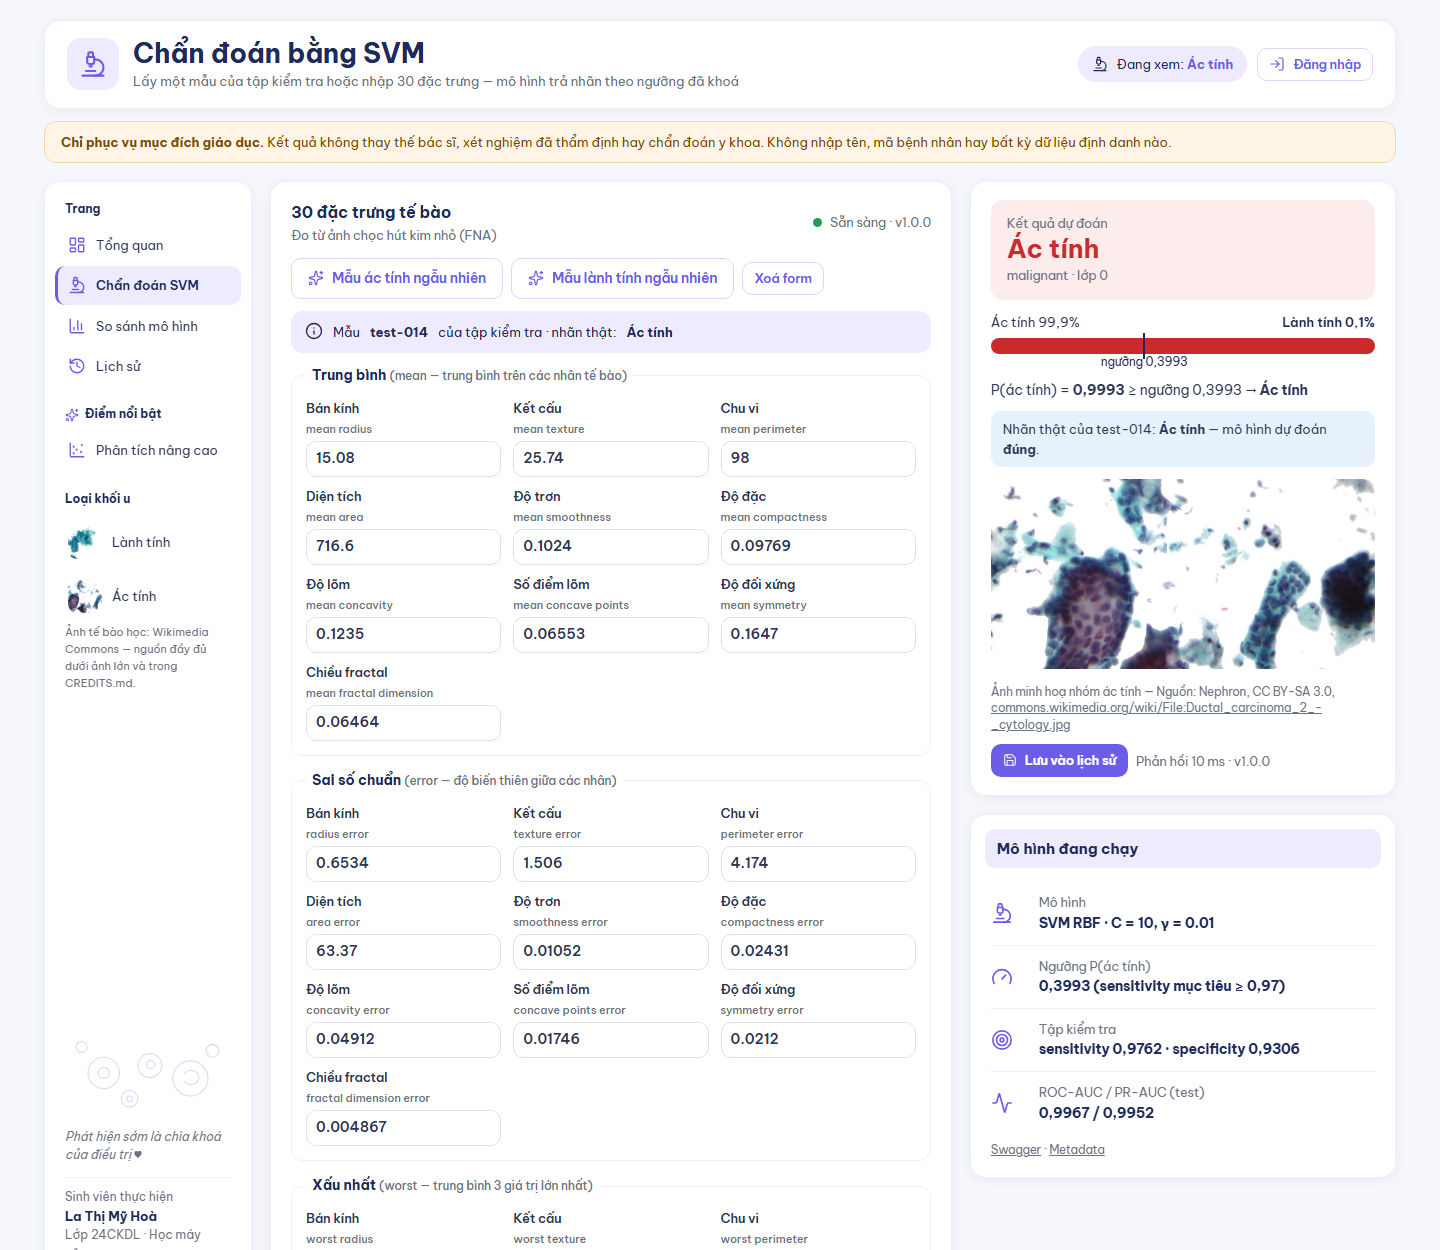
\includegraphics[width=\textwidth]{web_chan_doan.png}
\caption{Trang Chẩn đoán SVM: một mẫu ác tính của tập kiểm tra, dự đoán đúng}
\end{figure}

\subsection{Tài liệu API tương tác}
FastAPI sinh Swagger UI tại \texttt{/docs}: xem schema 30 trường, bấm \emph{Try it out}, gửi payload ví dụ (một mẫu
thật của tập kiểm tra) và quan sát mã trạng thái.

\begin{figure}[H]
\centering
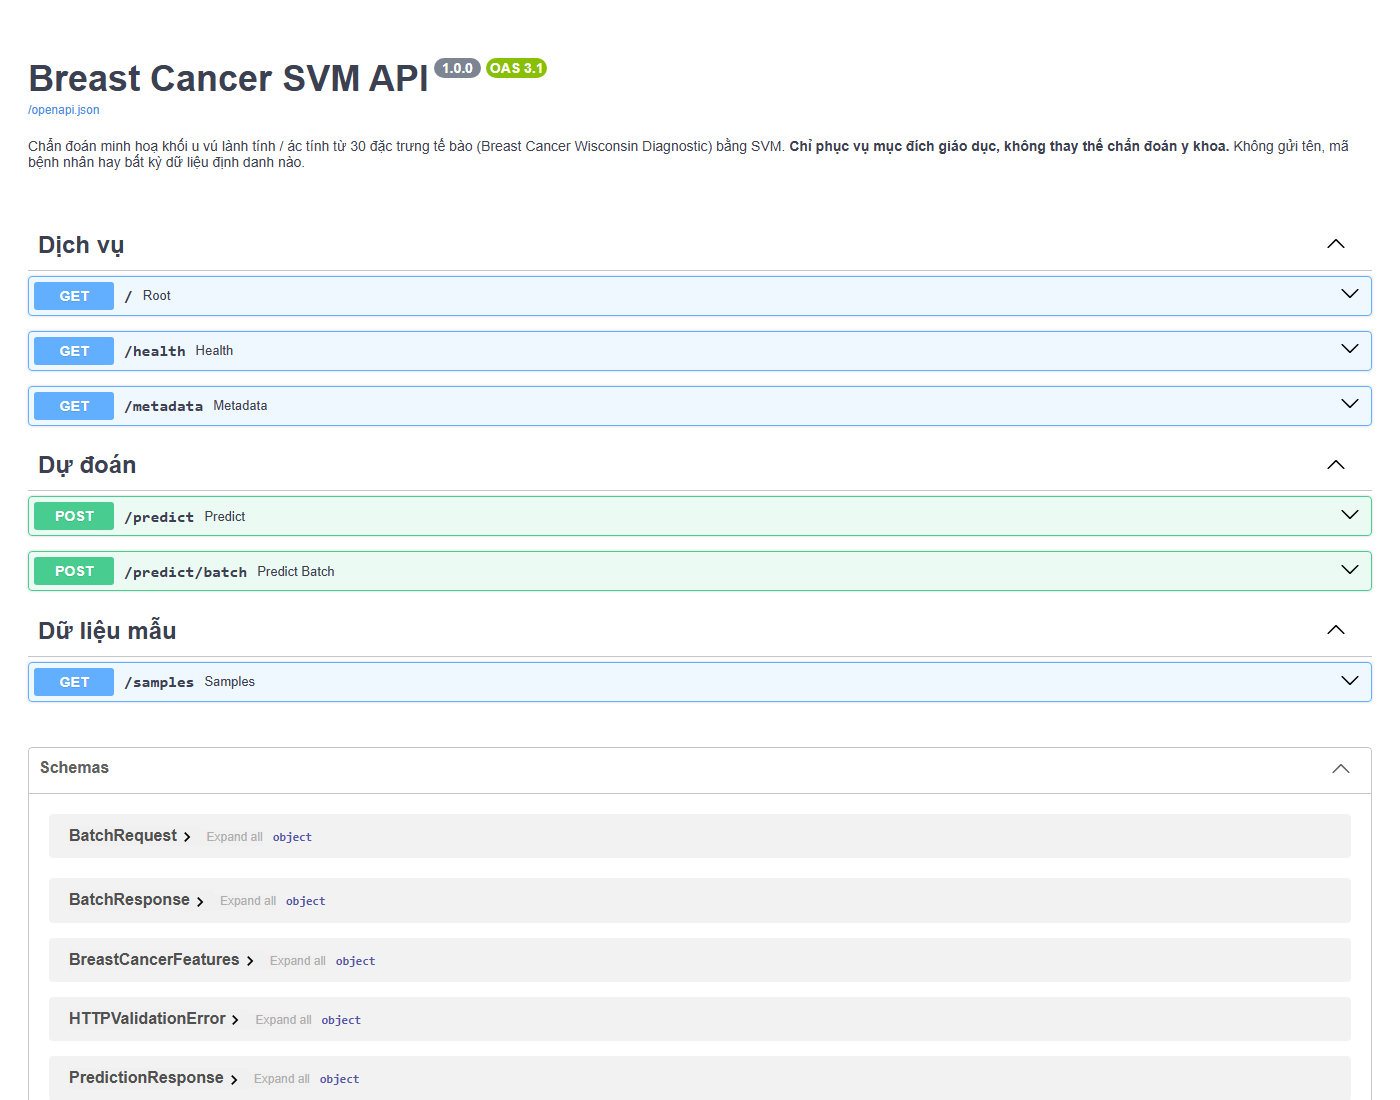
\includegraphics[width=0.9\textwidth]{swagger.png}
\caption{Swagger UI của dịch vụ}
\end{figure}

\subsection{Gọi API bằng curl}
\begin{lstlisting}[language=bash,numbers=none,caption={Dự đoán bằng curl với payload sinh từ dataset}]
python scripts/make_sample_request.py
curl -X POST "https://breast-cancer-svm-api-f2qq.onrender.com/predict" \
  -H "Content-Type: application/json" \
  -d @sample_request.json
\end{lstlisting}

\subsection{Gọi API bằng Python}
\begin{lstlisting}[caption={Lấy mẫu test rồi dự đoán bằng requests}]
import requests

BASE = "https://breast-cancer-svm-api-f2qq.onrender.com"
sample = requests.get(f"{BASE}/samples", params={"n": 1, "label": "malignant"}).json()["items"][0]
r = requests.post(f"{BASE}/predict", json={"features": sample["features"]}, timeout=60)
print(sample["label"], r.status_code, r.json()["predicted_label"], r.json()["probability_malignant"])
\end{lstlisting}

\subsection{Gọi API bằng JavaScript}
\begin{lstlisting}[language=java,numbers=none,caption={fetch trong trình duyệt}]
const base = "https://breast-cancer-svm-api-f2qq.onrender.com";
const { items } = await (await fetch(`${base}/samples?n=1&label=benign`)).json();
const res = await fetch(`${base}/predict`, {
  method: "POST",
  headers: { "Content-Type": "application/json" },
  body: JSON.stringify({ features: items[0].features }),
});
console.log(res.status, await res.json());
\end{lstlisting}

\subsection{Kết quả trả về}
\begin{lstlisting}[language={},numbers=none,caption={Phản hồi của /predict}]
{
  "predicted_class": 0,
  "predicted_label": "malignant",
  "predicted_label_vi": "...",
  "probability_malignant": 0.9971,
  "probability_benign": 0.0029,
  "threshold_malignant": 0.3993,
  "model_version": "1.0.0",
  "warning": "... Educational use only; not a medical diagnosis."
}
\end{lstlisting}
Phản hồi trên là của \texttt{sample\_request.json} (dòng 0 của dataset, nhãn thật ác tính); trường chữ tiếng Việt được
rút gọn. Gửi thiếu một trường sẽ nhận:
\begin{lstlisting}[language={},numbers=none,caption={Phản hồi 422 khi thiếu trường}]
{"detail": [{"type": "missing", "loc": ["body", "mean radius"], "msg": "Field required"}],
 "missing": ["mean radius"], "extra": []}
\end{lstlisting}

% =============================================================================
\section{Giới hạn và hướng phát triển}
% =============================================================================

\paragraph{Giới hạn.}
\begin{itemize}
  \item Dữ liệu \emph{một cơ sở}, \NSamples{} ca; chưa có đánh giá ngoại bộ trên quần thể, thiết bị hay quy trình khác.
  \item Tập test chỉ có \TestMalignant{} ca ác tính: mỗi ca bỏ sót đổi sensitivity khoảng 2,4 điểm phần trăm.
  \item Dữ liệu không có mã bệnh nhân nên không chia được theo bệnh nhân hay thời gian như dữ liệu bệnh viện thật cần.
  \item Đầu vào là 30 số đo trích sẵn; mô hình không đọc ảnh, không kiểm soát được chất lượng phép đo.
  \item Xác suất được hiệu chỉnh trên chính dữ liệu này; không có gì bảo đảm vẫn đúng ở nơi khác.
\end{itemize}

\paragraph{Hướng phát triển.} Đánh giá ngoại bộ đa cơ sở; chọn ngưỡng theo chi phí lâm sàng do chuyên gia xác định;
thêm giải thích dự đoán (ví dụ SHAP) để bác sĩ thấy đặc trưng nào đẩy xác suất lên; ghi nhận nhãn thật để giám sát
trôi dữ liệu và hiệu chỉnh lại; container hoá; thêm xác thực và rate limit nếu mở cho người dùng thật.

% =============================================================================
\section{Kết luận}
% =============================================================================

Sản phẩm hoàn thành chuỗi công việc từ dữ liệu tới dịch vụ trực tuyến theo đúng quy trình của bài giảng: chia tập
đúng cách, pipeline chuẩn hoá và SVM, đánh giá theo mục tiêu y khoa, artifact có phiên bản, API FastAPI có kiểm tra
đầu vào chặt, kiểm thử tự động, triển khai trên Render. Mô hình đạt sensitivity \TestSens{} và ROC-AUC \TestAUC{} trên
tập kiểm tra với ngưỡng \Threshold{} chọn trước trên dữ liệu kiểm định.

Bài học lớn nhất nằm ở ngưỡng và xác suất chứ không ở độ chính xác: một mô hình có ROC-AUC gần 1 vẫn phải chọn giữa
bỏ sót và báo động nhầm, và lựa chọn đó phải được đưa ra \emph{trước} khi nhìn tập kiểm tra. Cuối cùng, một API chạy
được không đồng nghĩa với một công cụ y tế sẵn sàng sử dụng: chất lượng dữ liệu, kiểm định ngoại bộ, hiệu chỉnh, bảo
mật và quản trị rủi ro là các phần bắt buộc của hệ thống thật.

% =============================================================================
\appendix
\section{Phụ lục: mã nguồn Python}
% =============================================================================

\subsection{scripts/train.py --- huấn luyện, hiệu chỉnh, chọn ngưỡng}
\lstinputlisting[language=Python]{../../scripts/train.py}

\subsection{app/main.py --- ứng dụng FastAPI}
\lstinputlisting[language=Python]{../../app/main.py}

\subsection{app/schemas.py --- schema 30 trường}
\lstinputlisting[language=Python]{../../app/schemas.py}

\subsection{app/model\_service.py --- nạp artifact và dự đoán theo ngưỡng}
\lstinputlisting[language=Python]{../../app/model_service.py}

\subsection{scripts/evaluate.py --- đánh giá và sinh hình}
\lstinputlisting[language=Python]{../../scripts/evaluate.py}

\subsection{scripts/smoke\_test.py --- kiểm tra sau triển khai}
\lstinputlisting[language=Python]{../../scripts/smoke_test.py}

\subsection{tests/test\_api.py --- ma trận kiểm thử}
\lstinputlisting[language=Python]{../../tests/test_api.py}

\subsection{app/comparison.py --- so sánh năm mô hình phân loại}
\lstinputlisting[language=Python]{../../app/comparison.py}

\subsection{db\_api/auth.py --- đăng ký, đăng nhập}
\lstinputlisting[language=Python]{../../db_api/auth.py}

\subsection{db\_api/history.py --- lịch sử dự đoán}
\lstinputlisting[language=Python]{../../db_api/history.py}

\subsection{db\_api/export.py --- xuất Excel}
\lstinputlisting[language=Python]{../../db_api/export.py}

\subsection{security.py --- bcrypt và JWT}
\lstinputlisting[language=Python]{../../security.py}

\subsection{Tệp cấu hình}
\lstinputlisting[caption={requirements.txt}]{../../requirements.txt}

\end{document}
